\documentclass[aspectratio=1610, polish]{beamer} 
% Jeśli chcesz otrzymać prezentację w języku polskim, to, powyżej, zamień „english” na „polish”
\usepackage{babel}
\makeatletter
\@ifclasswith{beamer}{polish}{
	\usepackage{polski}
}
\makeatother
\usepackage[utf8]{inputenc}
\usepackage{listings} % We want to put listings
% \usepackage{minted}   % We want to put listings

\mode<beamer>{ 	% In the 'beamer' mode
	\hypersetup{pdfpagemode=FullScreen}         % Enable Full screen mode
	\usetheme[parttitle=rightfooter, nosidebar, margins=1em]{AGH}       % Show part title in right footer
	%\usetheme[nosidebar]{AGH}                  % Do not show sidebar on non-title slides
	% \usetheme[nosidebar, margins=1em]{AGH}     % Do not show sidebar on non-title slides and set both margins (left / right) to 1em
	%\usetheme[dark]{AGH}                       % Use dark background
	%\usetheme[dark, parttitle=leftfooter]{AGH} % Use dark background and show part title in left footer
}
\mode<handout>{	% In the 'handout' mode
	\hypersetup{pdfpagemode=None}		
	\usepackage{pgfpages}
	\pgfpagesuselayout{4 on 1}[a4paper,border shrink=5mm,landscape]	% Show 4 slides on 1 page
	\pgfpageslogicalpageoptions{1}{border code=\pgfusepath{stroke}}
	\pgfpageslogicalpageoptions{2}{border code=\pgfusepath{stroke}}
	\pgfpageslogicalpageoptions{3}{border code=\pgfusepath{stroke}}
	\pgfpageslogicalpageoptions{4}{border code=\pgfusepath{stroke}}
  	\usetheme{boxes}
  	\addheadbox{structure}{\quad\insertpart\hfill\insertsection\hfill\insertsubsection\qquad}          % Content of header
 	\addfootbox{structure}{\quad\insertshortauthor\hfill\insertframenumber\hfill\insertsubtitle\qquad} % Content of footer
}

\AtBeginPart{ % At begin part: display its name
	\frame{\partpage}
} 
\author[Beata Trzpil-Jurgielewicz]{mgr inż. Beata \textsc{Trzpil-Jurgielewicz}
\newline 
promotorzy:
\newline
prof. dr hab. inż. Władysław \textsc{Dąbrowski} 
\newline 
dr inż. Paweł \textsc{Hottowy}}
\date{}
\iflanguage{polish}
{
	\title[]{Opracowanie wielokanałowego układu scalonego w technologii CMOS do rejestracji aktywności neuronalnej oraz jego aplikacja w funkcjonalnych badaniach mózgu
	}
	% \institute[AGH]{
	% 		\inst{1}Instytut Informatyki\newline
	% 		ul. Kawiory 21\newline
	% 		30-055 Kraków\newline
	% 		\url{http://www.icsr.agh.edu.pl/~polak/}
	% 	\and
	% 		\inst{2}Druga afiliacja
 	% }
}{
	\title{---}
	% \institute[AGH]{
	% 		\inst{1}Institute of Computer Science\newline
	% 		Kawiory 21 Street\newline
	% 		30-055 Kraków\newline
	% 		Poland\newline
	% 		\url{http://www.icsr.agh.edu.pl/~polak/}
	% 	\and
	% 		\inst{2}Second affiliation
	% }
}
%%%%%%%%%%% Configuration of the listings package %%%%%%%%%%%%%%%%%%%%%%%%%%
% Source: https://en.wikibooks.org/wiki/LaTeX/Source_Code_Listings#Using_the_listings_package
%%%%%%%%%%%%%%%%%%%%%%%%%%%%%%%%%%%%%%%%%%%%%%%%%%%%%%%%%%%%%%%%%%%%%%%%%%%%
\lstset{ %
  backgroundcolor=\color{white},   % choose the background color
  basicstyle=\footnotesize,        % the size of the fonts that are used for the code
  breakatwhitespace=false,         % sets if automatic breaks should only happen at whitespace
  breaklines=true,                 % sets automatic line breaking
  captionpos=b,                    % sets the caption-position to bottom
  commentstyle=\color{green},      % comment style
  deletekeywords={...},            % if you want to delete keywords from the given language
  escapeinside={\%*}{*)},          % if you want to add LaTeX within your code
  extendedchars=true,              % lets you use non-ASCII characters; for 8-bits encodings only, does not work with UTF-8
  frame=single,	                   % adds a frame around the code
  keepspaces=true,                 % keeps spaces in text, useful for keeping indentation of code (possibly needs columns=flexible)
  keywordstyle=\color{blue},       % keyword style
  morekeywords={*,...},            % if you want to add more keywords to the set
  numbers=left,                    % where to put the line-numbers; possible values are (none, left, right)
  numbersep=5pt,                   % how far the line-numbers are from the code
  numberstyle=\tiny\color{gray},   % the style that is used for the line-numbers
  rulecolor=\color{black},         % if not set, the frame-color may be changed on line-breaks within not-black text (e.g. comments (green here))
  showspaces=false,                % show spaces everywhere adding particular underscores; it overrides 'showstringspaces'
  showstringspaces=false,          % underline spaces within strings only
  showtabs=false,                  % show tabs within strings adding particular underscores
  stepnumber=2,                    % the step between two line-numbers. If it's 1, each line will be numbered
  stringstyle=\color{cyan},        % string literal style
  tabsize=2,	                   % sets default tabsize to 2 spaces
  title=\lstname,                  % show the filename of files included with \lstinputlisting; also try caption instead of title
                                   % needed if you want to use UTF-8 Polish chars
  literate={ą}{{\k{a}}}1
           {Ą}{{\k{A}}}1
           {ę}{{\k{e}}}1
           {Ę}{{\k{E}}}1
           {ó}{{\'o}}1
           {Ó}{{\'O}}1
           {ś}{{\'s}}1
           {Ś}{{\'S}}1
           {ł}{{\l{}}}1
           {Ł}{{\L{}}}1
           {ż}{{\.z}}1
           {Ż}{{\.Z}}1
           {ź}{{\'z}}1
           {Ź}{{\'Z}}1
           {ć}{{\'c}}1
           {Ć}{{\'C}}1
           {ń}{{\'n}}1
           {Ń}{{\'N}}1
}
\usepackage{booktabs}
\usepackage{siunitx}
\sisetup{locale = PL,
         exponent-product=\ensuremath{\times}}
\graphicspath{{../PhD_Thesis_BTJ/Figures/}}
% \graphicspath{{../BTJ_Thesis/Figures/}}

\usepackage{caption}
\usepackage{subcaption}
\usepackage{tabularray}

\usepackage[most]{tcolorbox}    	% for COLORED BOXES (tikz and xcolor included)
\usepackage{ninecolors}
\selectcolormodel{rgb}
\definecolor{main}{HTML}{1F77B4}    % setting main color to be used
\definecolor{sub}{HTML}{cde4ff}     % setting sub color to be used
\definecolor{deepblue}{HTML}{1F77B4}
\definecolor{deepred}{HTML}{D92728}
\definecolor{lightred}{HTML}{D98789}
\definecolor{deepgreen}{HTML}{2CA02C}

\tcbset{
    sharp corners,
    colback = white,
    before skip = 0.2cm,    % add extra space before the box
    after skip = 0.5cm      % add extra space after the box
}  

\newtcolorbox{boxR}{
    enhanced, % for a fancier setting,
    boxrule = 0pt, % clearing the default rule
    borderline = {0.75pt}{0pt}{deepred}, % outer line
    borderline = {0.75pt}{2pt}{lightred}, % inner line
    % title = sda
}

\newcommand{\af}{dr hab. Andrzej Pfitzner, prof. PW}
\newcommand{\tb}{dr hab. inż. Teodor Buchner}
\newcommand{\dk}{dr hab. inż. Dariusz Komorowski, prof. PŚ}
\newcommand{\cit}[1]{\textit{[...]#1}}
\newcommand{\high}[1]{\textbf{#1}}

%%%%%%%%%%% Configuration of the minted package %%%%%%%%%%%%%%%%%%%%%%%%%%
% \setminted[C++]{frame=single,linenos}

%%%%%%%%%%%%%%%%%
\begin{document}
\maketitle


% \part{Tematyka pracy}
\begin{frame}{Plan prezentacji}
	\tableofcontents%[pausesections]
\end{frame}
\section{Systemy do rejestracji aktywności elektrycznej żywych tkanek nerwowych}
\section{Projekt liniowego pseudo-rezystora w zakresie \si{\giga\ohm}}
\section{Operacyjny wzmacniacz transkonduktancyjny}
\section{Weryfikacja elektroniczna i neurofizjologiczna układu scalonego HiFiNeuroPre}

\part{Tematyka pracy}
\begin{frame}{Cele pracy}

    \begin{alertblock}{}
        Celem projektu przedstawionego w niniejszej pracy było opracowanie i weryfikacja koncepcji przedwzmacniacza dedykowanego do wielokanałowej sondy neuronalnej umożliwiającej rejestrację aktywności neuronalnej mózgu.
    \end{alertblock}

    \begin{block}{Główne zadania}
        \begin{itemize}
            \item Kompleksowa analiza zniekształceń nieliniowych we wzmacniaczach neuronalnych
            \item Optymalizacja kluczowych parametrów przedwzmacniaczy neuronalnych
            \item  Projekt układu scalonego, obwodu drukowanego oraz systemu akwizycji danych
            \item Wykonanie testów elektronicznych oraz analiza parametrów i charakterystyk opracowanego układu scalonego
            \item Weryfikacja funkcjonalności opracowanego przedwzmacniacza  w eksperymentach neurobiologicznych i analiza zebranych danych
        \end{itemize}
    \end{block}

    
\end{frame}

\begin{frame}{Zakresy amplitud i częstotliwości sygnałów neuronowych w różnych technikach rejestracji}
    \begin{columns}
        \column{.48\textwidth}
        \vspace{-2em}

        \begin{figure}[H]
            \includegraphics[scale=0.2]{ch1/brain.jpg}
          \end{figure}

          \begin{block}{Metody rejestracji}
            \begin{itemize}
                {\renewcommand\normalsize{\small}%
                \normalsize
                \item LFP -- Local Field Potential
                \item AP --  Action Potential
                \item ECoG -- Electrocorticography
                \item EEG -- Electroencephalography
                }
            \end{itemize}
        \end{block}


        \column{.48\textwidth}
        \vspace{-2em}

        \begin{figure}[H]
            \centering
            \includegraphics[scale=1.0]{ch1/lfp_ap_spectrum}  
            \end{figure}	
    \end{columns}
    
\end{frame}

\begin{frame}{Kierunki rozwoju współczesnych systemów pomiarowych i matryc mikroelektrodowych}
   
    \begin{columns}
    \column{.55\textwidth}

    \begin{block}{Techniki pomiarowe wewnątrz i \\
        zewnątrzkomórkowe w neurobiologii}
        \begin{itemize}
            \item różne amplitudy sygnałów
            \item inwazyjność badań
            \item obszar badań 
        \end{itemize}
    \end{block}
    \column{.4\textwidth}
    \vspace{-3em} %5mm vertical space

        \begin{columns}
        \column{.5\textwidth}
        \begin{figure}[H]
            \includegraphics[scale=0.13]{ch2/masm64Dsharp.png}
        \end{figure}

        \column{.5\textwidth}
            \begin{figure}[H]
                \includegraphics[scale=0.13]{ch2/utahArr.png}
            \end{figure}
        \end{columns}
    \end{columns}

    \begin{columns}

        \column{.55\textwidth}
        % \vspace{-3em} %5mm vertical space

        \begin{figure}[H]
            \includegraphics[scale=0.45]{ch1/intra-extra.png}  
        \end{figure}

        \column{.4\textwidth}
        \vspace{-2em} %5mm vertical space
        \begin{figure}[H]
                % \includegraphics[scale=0.25]{ch1/ap.png}
            \includegraphics[scale=0.25]{ch2/neuropixel10.png}  
        \end{figure}


    \end{columns}


    
\end{frame}

% \begin{frame}{Kierunki rozwoju współczesnych systemów pomiarowych i matryc mikroelektrodowych}
%     \vspace{-5mm} %5mm vertical space

%     \begin{columns}[t]
%         \column{.3\textwidth}
%         \begin{figure}[H]
%             \includegraphics[scale=0.35]{ch2/neuropixel10.png}  
%         \end{figure}

%         \column{.3\textwidth}
%         \begin{figure}[H]
%             \includegraphics[scale=0.35]{ch2/argo.jpeg}  
%         \end{figure}

%         \column{.35\textwidth}
%         \begin{figure}[H]
%             \includegraphics[scale=0.2]{ch2/masm64Dsharp.png}
%         \end{figure}

%         \begin{figure}[H]
%             \includegraphics[scale=0.25]{ch2/utahArr.png}
%         \end{figure}

%     \end{columns}


% \end{frame}





\begin{frame}{Kanał rejestracji neuronowej z wykorzystaniem mikroelektrod zewnątrzkomórkowych}
\vspace{-1em}
    \begin{columns}
        \column{.48\textwidth}
        \begin{figure}[H]
            \centering
            \includegraphics[scale=0.25]{ch2/chemNeuroInterface.png} 

        \end{figure}
        \begin{figure}[H]
            \centering
            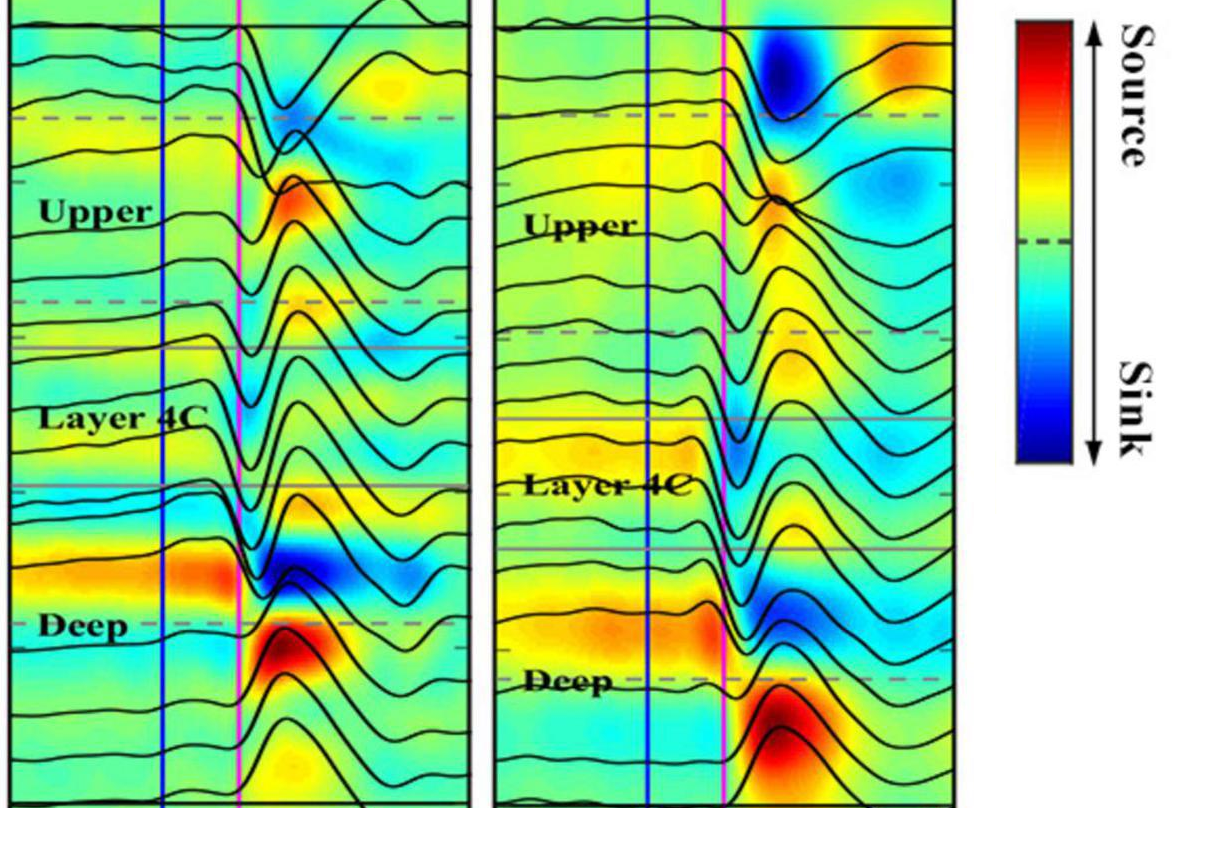
\includegraphics[scale=0.25]{ch1/lfp.png} 

          \end{figure}

        \column{.48\textwidth}
        \begin{block}{Wymagania stawiane interfejsom neuroelektronicznym umożliwiającym rejestrację sygnałów LFP i AP}
            \begin{itemize}
                \item Stałe napięcie na styku elektrody -- do $\SIrange{1}{2}{\volt}$ 
                \item Szumy $<\SI{10}{\micro\volt}$ dla pasma LFP i AP
                \item Liniowość rejestrowanego sygnału
                \item Pobór mocy -- limit ogrzewania tkanki mózgowej --  mniej niż  $\SI{1}{\degreeCelsius}$ 
                \item Zróżnicowane sygnały: amplituda do $\SI{10}{\milli\volt_{pp}}$ dla LFP i od  $\SI{50}{\micro\volt}$ dla AP
                \item Skalowalność -- tysiące kanałów dla przyszłych systemów
            \end{itemize}
        \end{block}
        % Schemat typowego kanału rejestracji neuronowej i modelu elektrycznego interfejsu tkanka-mikroelektroda: 
        % $Z_{CPA}$ -- element o stałej fazie, 
        % $R_{CT}$ -- rezystancja dla przepływającego prądu przez elektrodę,  
        % $R_{SP}$ -- rezystancja rozproszona elektrolitu, 
        % $V_{HC}$ -- potencjał w interfejsie elektroda -- tkanka. 
 
    \end{columns}
\end{frame}


% \begin{frame}{Sprzężenie zmiennoprądowe}
%     \begin{columns}
%         \column{.48\textwidth}

%     \begin{figure}[H]
%         \centering
%         \includegraphics[scale=0.75]{ch2/conceptAC_Harrison.pdf} 
%     \end{figure}
%     \column{.48\textwidth}
%     \begin{alertblock}{Wyzwania zwiazane z sprzęzeniem AC}
%         \begin{itemize}
%             \item Niska dolna częstotliwość graniczna rzędu~$\SI{\sim 1}{\hertz}$ 
%             \item Pojemności w technologi CMOS są rzędu $\SI{}{\femto\farad\per\micro\metre\squared}$
%             \item Rezystancja sprzężenia zwrotnego w zakresie $\SI{}{\tera\ohm}$
%         \end{itemize}
%     \end{alertblock}
%     \begin{exampleblock}{Zalety}
%         \begin{itemize}
%             \item Usunięcie składowej stałej od elektrody niezależnie od jej wartości
%             \item Wydajność szumowa i poboru mocy
%         \end{itemize}
%     \end{exampleblock}
% \end{columns}

% \end{frame}



% \begin{frame}{Sprzężenie stałoprądowe}
%     \begin{columns}
%         \column{.48\textwidth}
%         \begin{figure}[H]
%             \centering
%             \includegraphics[scale = 0.5]{ch2/dc_coupling.pdf}
%         \end{figure}

%     \column{.48\textwidth}
%     \begin{alertblock}{Wyzwania zwiazane z sprzęzeniem DC}
%         \begin{itemize}
%             \item Duża wrażliwość na offset
%             \item Pobór mocy
%         \end{itemize}
%     \end{alertblock}
%     \begin{exampleblock}{Zalety}
%         \begin{itemize}
%             \item Brak konieczności używania dużych rezystancji w pętli sprzężenia zwrotnego
%         \end{itemize}

%         \begin{figure}[H]
%             \centering
%             \includegraphics[scale=0.5]{ch2/dc-integrator.pdf} 
%         \end{figure}

%     \end{exampleblock}
% \end{columns}

% \end{frame}

\begin{frame}{Sprzężenie zmiennoprądowe i stałoprądowe}
    

    \begin{columns}
        \column{.55\textwidth}
        \vspace{-1em} %5mm vertical space

        \begin{figure}[H]
            \centering
            \includegraphics[scale=0.5]{ch2/conceptAC_Harrison.pdf} 
        \end{figure}
        \vspace{-2em} %5mm vertical space

        {\renewcommand\normalsize{\small}%
        \normalsize
    
        % \begin{alertblock}{Wyzwania zwiazane z sprzęzeniem AC}
    %5mm vertical space
    
        % \begin{exampleblock}{Zalety}
        % \begin{exampleblock}{Sprzężenie zmiennoprądowe}
        \begin{exampleblock}{}

            \begin{itemize}
                \item Całkowite usunięcie napięcia stałego na elektrodzie 
                \item Konieczność implementacji filtru górnoprzepustowego z dolną częstotliwością graniczną rzędu~$\SI{\sim 1}{\hertz}$ 
                \item Ograniczenia na pojemności kondensatorów w technologii CMOS ~pF $\sim\SI{}{\pico\farad}$
                \item  Wymagane rezystancje  $\sim\SI{}{\tera\ohm}$
            \end{itemize}
        \end{exampleblock}
    
        }


        \column{.43\textwidth}
        \vspace{-3em} %5mm vertical space

        \begin{figure}[H]
            \hspace{-2em} %5mm vertical space
            \includegraphics[scale = 0.48]{ch2/dc_coupling.pdf}
        \end{figure}


    {\renewcommand\normalsize{\small}%
    \normalsize
    % \begin{alertblock}{Wyzwania zwiazane z sprzęzeniem DC}
    \vspace{-1em} %5mm vertical space

    % \begin{alertblock}{Sprzężenie stałoprądowe}
        \begin{alertblock}{}

        \begin{itemize}
            \item Alternatywne podejście do eliminacji składowej stałej napięcia na styku elektrody i tkanki
        \end{itemize}
    \end{alertblock}
    }

    \end{columns}

\end{frame}


\part{Liniowy pseudo-rezystor}


% \begin{frame}{Podstawowe rozwiązania psuedo-rezystorów}


%         \begin{figure}[H]
%             \centering
%             \includegraphics[scale = 0.6]{ch2/ntpr.pdf}

%         \end{figure}
%         \vspace{-5mm} %5mm vertical space
%         % Różne topologie pseudo-rezystorów z niekontrolowaną wartością rezystancji zaimplementowane w przedwzmacniaczu ze sprzężeniem zmiennoprądowym.        
%         \begin{alertblock}{Wady}
%             \begin{itemize}
%                 \item stała rezystancja 
%                 \item brak możliwości regulacji częstotliwości granicznej
%             \end{itemize}
%         \end{alertblock}



% \end{frame}

% \begin{frame}{Podstawowe rozwiązania psuedo-rezystorów - regulowana wartość rezystancji}
%     \begin{block}{}
%         Regulacja częstotliowści granicznej
%     \end{block}

%     \begin{columns}
%         \column{.58\textwidth}
%         \hspace{-10mm} %5mm vertical space
%         \begin{figure}[H]

%             \includegraphics[scale = 0.6]{ch2/tpr.pdf}

%         \end{figure}
%         \column{.35\textwidth}
%         % Różne topologie pseudo-rezystorów z kontrolowaną wartością rezystancji zaimplementowane w przedwzmacniaczu ze sprzężeniem zmiennoprądowym.
%         \vspace{-5mm} \begin{alertblock}{}
%         Zmieniające się napięcie panujące pomiędzy bramką a źródłem tranzystora w zależności od sygnału wejściowego
%         \end{alertblock}
%         \vspace{5mm} 
%         \begin{exampleblock}{}
%             Zachowanie stałego napięcia pomiędzy bramką, a źródłem niezależnie od sygnału wejsciowego 

%         \end{exampleblock}
%     \end{columns}


% \end{frame}


\begin{frame}{Podstawowe rozwiązania psuedo-rezystorów}
    \vspace{-1em}
    \begin{block}{}
        Zastosowanie tranzystorów jako elementów rezystancjach, zwanych pseudo-rezystorami, jest powszechną praktyką w projektowaniu obwodów analogowych dla przypadków, w których bierne rezystory nie są odpowiednie ze względu na wartości wymaganych rezystancji lub powierzchnie takich elementów. 
       \end{block}
    \begin{columns}
        \column{.48\textwidth}
        \vspace{-2em}
        \begin{figure}[H]
            \includegraphics[scale = 0.4]{ch2/ntpr.pdf}
        \end{figure}
        \begin{alertblock}{}
            brak możliwości regulacji wartości rezystancji
        \end{alertblock}



        \column{.48\textwidth}
        \begin{figure}[H]
            \includegraphics[scale = 0.4]{ch2/tpr.pdf}
        \end{figure}
        \vspace{-1em}
        \begin{exampleblock}{}
            możliwość regulacji wartości rezystancji za pomocą modyfikacji napięcia panującego na bramce tranzystora
        \end{exampleblock}

    \end{columns}
\end{frame}








% \begin{frame}{Analiza stałoprądowa}

        
%     \vspace{-1em}


%     \begin{columns}
%         \column{.48\textwidth}
%          \begin{alertblock}{}
%             \begin{figure}[H]
%                 \includegraphics[scale=0.8]{ch3/ptune.pdf}
%             \end{figure}
%             \end{alertblock}
%         \column{.48\textwidth}
%         \begin{exampleblock}{}
%             \begin{figure}[H]
%                 \includegraphics[scale=0.8]{ch3/pvgs.pdf}
%             \end{figure}

%         \end{exampleblock}
%     \end{columns}

% \vspace{-0.5em}
%     \begin{columns}
%         \column{.48\textwidth}
%         \begin{figure}[H]
%             \centering
%             \includegraphics[scale = 0.7]{scripts/tmp/pseudoresistors_IV.pdf}
%                 \end{figure}
%         \column{.48\textwidth}
%         \begin{figure}[H]
%             \centering
%             \includegraphics [scale = 0.7]{scripts/tmp/pseudoresistors_R.pdf}
%         \end{figure}
%     \end{columns}


% \end{frame}

\begin{frame}{Architektura wzmacniacza neuronowego wykorzystującego sprzężenie zmiennoprądowe w różnych implementacjach pseudo-rezystorów}
    \begin{columns}[t]

        \column{.5\textwidth}
        \vspace{-2em} %5mm vertical space

        \begin{alertblock}{Zmieniające się napięcie  pomiędzy bramką a źródłem tranzystora w zależności od sygnału wejściowego -- $variable-V_{gs}$}
                 

            \begin{figure}[H]
                \centering
                \includegraphics[scale = 0.75]{ch3/fig1-ac_standard.pdf}
            \end{figure}
        \end{alertblock}



        \column{.45\textwidth}
        \vspace{-2em} %5mm vertical space

        \begin{exampleblock}{Słałe napięcia pomiędzy bramką, a źródłem niezależnie od sygnału wejsciowego -- $fixed-V_{gs}$}
            \begin{figure}[H]
                \centering
                \includegraphics[scale = 0.75]{ch3/fig1-ac_work_simplicite}
            \end{figure}
        \end{exampleblock}

    \end{columns}
\end{frame}

\begin{frame}{Analiza liniowości pseudo-rezystorów}
    \vspace{-1em}



    \begin{columns}
        \column{.33\textwidth}
        \begin{block}{Ustawienia symulacji}
            \begin{itemize}
                \item Badanie odpowiedzi układu  w dziedzinie czasu na wymuszenia sinusoidalne
                \item Częstotliwość graniczna dla układów z sprzężeniem AC $\SI{\sim 1}{\hertz}$
                \item Analiza: Transformata Fouriera -- wyznaczenie współczynnika THD -- miara liniowości rejestrowanego sygnału
                \item $\mathrm{THD} = \frac{\sqrt{\sum_{n=2}^{+\infty} U_k^2}}{U_1}$
                % \item Amplitudy poszczególnych harmonicznych 
            \end{itemize}
                \end{block}
        \column{.32\textwidth}
        \vspace{-1em} %5mm vertical space
        \begin{alertblock}{$variable-V_{gs}$}
        \begin{figure}[H]
            \centering
            \includegraphics[scale = 0.65]{scripts/tranTHDAmp/tranTHDAmp_ner.pdf}
        \end{figure}
    \end{alertblock}
        \column{.32\textwidth}
        \vspace{-1em} %5mm vertical space
        \begin{exampleblock}{$fixed-V_{gs}$}
        \begin{figure}[H]
            \centering
            \includegraphics[scale = 0.65]{scripts/tranTHDAmp/tranTHDAmp_pr_sim.pdf}
        \end{figure}
    \end{exampleblock}
    \end{columns}

\end{frame}



% \begin{frame}{Projekt przedwzmacniacza z modelem pseudo-rezystora w technologii $\SI{180}{\nano\metre}$  XFAB}
%     \begin{figure}[H]
%         \centering
%         \includegraphics[scale=1.0]{ch3/pseudo-lay.pdf} 

%     \end{figure}


% \end{frame}

% \begin{frame}{Wpływ pojemnościowych prądów bramki pseudo-rezystorów na zniekształcenia  w technologii $\SI{180}{\nano\metre}$}
%     \vspace{-5mm} %5mm vertical space

%     \begin{columns}
%         \column{.3\textwidth}
%         \begin{figure}[H]

%             \includegraphics[trim={0 0.25cm 0 0.25cm}, clip, scale = 0.6]{scripts/tmp/IdsA.pdf}

%         \end{figure}
%         \column{.3\textwidth}
%         \begin{figure}[H]

%             \includegraphics[trim={0 0.25cm 0 0.25cm}, clip, scale = 0.6]{scripts/tmp/IdsB.pdf}

%         \end{figure}
%         \column{.3\textwidth}
%         \begin{figure}[H]

%             \includegraphics[trim={0 0.25cm 0 0.25cm}, clip, scale = 0.6]{scripts/tmp/IgbA.pdf}

%         \end{figure}

%     \end{columns}
%     \vspace{-10mm} %5mm vertical space
%     \begin{columns}
%         \column{.3\textwidth}
%         \begin{figure}[H]

%             \includegraphics[trim={0 0.25cm 0 0.25cm}, clip, scale = 0.6]{scripts/tmp/IgbB.pdf}

%         \end{figure}
%         \column{.3\textwidth}
%         \begin{figure}[H]

%             \includegraphics[trim={0 0.25cm 0 0.25cm}, clip, scale = 0.6]{scripts/tmp/vOut.pdf}

%         \end{figure}
%         \column{.3\textwidth}
%         \begin{figure}[H]

%             \includegraphics[trim={0 0.25cm 0 0.25cm}, clip, scale = 0.6]{scripts/tmp/Igb_diff.pdf}

%         \end{figure}

%     \end{columns}
        



% \end{frame}


% \begin{frame}{Skalowanie zniekształceń z powierzchnią bramki i grubością tlenku tranzystorów tworzących pseudo-rezystory}
%     \begin{columns}
%         \column{.48\textwidth}
%         \begin{block}{Powierzchnia bramki -- technologia $\SI{180}{\nano\metre}$ }
%             \begin{figure}[H]
%                 \centering
%                 \includegraphics[scale = 0.7]{scripts/analyseTran/analyseTranSize.pdf}
%             \end{figure}
%         \end{block}

%         \column{.48\textwidth}
%         \begin{block}{Zależnosć od technologii}
%             \begin{figure}[H]
%                 \centering
%                 \includegraphics[scale = 0.7]{scripts/analyseTran/analyseTranTechnology.pdf}
%             \end{figure}
%         \end{block}


%     \end{columns}

% \end{frame}

% \begin{frame}{Szumy}
%     \vspace{-5mm} %5mm vertical space

%     \begin{columns}
%     \column{.3\textwidth}
%     \begin{figure}[H]
%         \centering
%         \includegraphics[scale=0.5]{ch2/conceptAC_Harrison.pdf} 
%     \end{figure}
%         \column{.3\textwidth}
%         \begin{figure}[H]
%             \centering
%             \includegraphics[scale = 0.5]{scripts/tmp/fig3_R1.pdf}
%         \end{figure}
%         \column{.3\textwidth}
%         \begin{figure}[H]
%             \centering
%             \includegraphics[scale = 0.5]{scripts/tmp/fig3_R2.pdf}
%         \end{figure}
%     \end{columns}

%     \vspace{-5mm} %5mm vertical space


%     \begin{columns}
%         \column{.3\textwidth}
%         \begin{figure}[H]
%             \centering
%             \includegraphics[scale=0.5]{scripts/noiseOutResistors/fig1_R1.pdf}
%         \end{figure}
%         \column{.3\textwidth}
%         \begin{figure}[H]
%             \centering
%             \includegraphics[scale=0.5]{scripts/noiseOutResistors/fig2.pdf}
%         \end{figure}
%     \end{columns}


% \end{frame}


\begin{frame}{Wpływ pojemności wejściowych na szumy i zniekształcenia}
    \begin{columns}
        \column{.49\textwidth}
        \vspace{-1em}

        \begin{figure}[H]
            \centering
            \includegraphics[scale=0.45]{ch2/conceptAC_Harrison.pdf} 
        \end{figure}
\vspace{-2em}

        \begin{block}{Parametry}
            \begin{itemize}
                \item Różne wartości $C_{in}$, oraz $C_{f}$ przy stałym stosunku wzmocnienia $Gain = \SI{20}{\volt\per\volt}$
                \item Wartości $R_{f}$ dostoswane dla każdej symulacji niezależnie tak, aby uzyskać tę samą częstotliwość graniczną $\SI{1}{\hertz}$
                \item Ekwiwalentne szumy wejściowe mierzone w paśmie $\SI{1}{\hertz}$ -- $\SI{10}{\kilo\hertz}$
            \end{itemize}
                \end{block}

            \column{.5\textwidth}

    \begin{figure}[H]
        \centering
        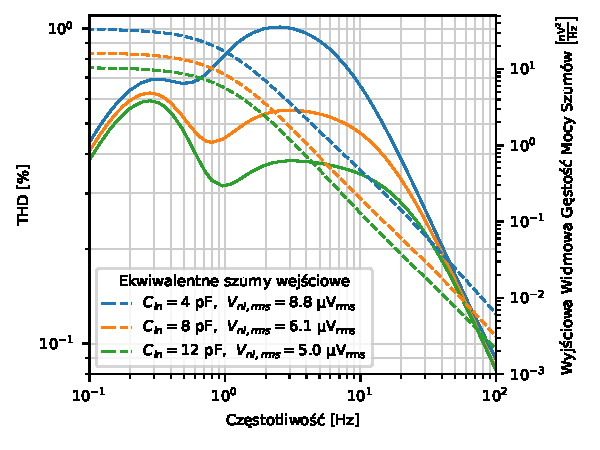
\includegraphics[scale=0.8]{scripts/tmp/thd_C_in.pdf} 
    \end{figure}
\end{columns}

\end{frame}


\part{Operacyjny wzmacniacz transkonduktancyjny}
% \begin{frame}{Implementacja teleskopowej kaskody ze zintegrowanym sprzężeniem AC}
%     \begin{columns}

%         \column{.6\textwidth}
%         \begin{figure}[H]
%             \includegraphics[scale = 0.75]{ch4/chap4Scheme.pdf} 
%         \end{figure}

%         \column{.35\textwidth}


%         \begin{block}{Kluczowe wymagnia}
%         \begin{itemize}
%             \item optymalizacja szumowa
%             \item powierzchnia
%             \item pobór mocy
%         \end{itemize}
%             \end{block}



%     \end{columns}   
%  \end{frame}



% \begin{frame}{Analiza szumowa pary różnicowej}
%     \begin{figure}[H]
%         \centering
%         \includegraphics[scale = 0.75]{scripts/tmp/differentialPair.pdf}  
%     \end{figure}

% \end{frame}



\begin{frame}{Przedwzmacniacz z wejściowym obwodem sprzęgającym AC}
    \begin{columns}

    \column{.65\textwidth}
    \begin{figure}[H]
        \centering
        \includegraphics[scale=0.45]{ch4/channel.pdf} 
    \end{figure}   

    \column{.35\textwidth}

    \begin{block}{
    }
    {\renewcommand\normalsize{\small}%
    \normalsize
    \begin{itemize}
        \item Konfiguracja  teleskopowej kaskody  jako aktywny OTA
        \item Polaryzacja pary różnicowej w obszarze podprogowym pracy tranzystora
        \item  Napięcie zasilania $\SI{\pm 1.8}{\volt}$
    \end{itemize}
    \vspace{-1em}
    \begin{table}[H]
        \centering
        \begin{tabular}{lll} 
        \toprule
        \begin{tabular}[c]{@{}l@{}}Kluczowe \\tranzystory\end{tabular} & $W$ [$\SI{}{\micro\metre}$] & $L$ [$\SI{}{\micro\metre}$]  \\ 
        \toprule
        $M_{bias}$                                                       & 10                          & 10                           \\
        $M_1,\ M_2$                                                    & 300                         & 1                            \\
        $M_3,\ M_4$                                                    & 20                          & 2                            \\
        $M_5,\ M_6$                                                    & 5                           & 5                            \\
        $M_7,\ M_8$                                                    & 4                           & 48                           \\
        \bottomrule
        \end{tabular}
    \end{table}
    }
    \end{block}
    \end{columns}   
  
\end{frame}


% \begin{frame}{Blok korekcji}
% \begin{columns}

%     \column{.35\textwidth}
%     \begin{block}{
%         Projekt kanału}
%         \begin{figure}[H]
%             \centering
%             \includegraphics[scale = 0.4]{ch4/chap4Scheme.pdf}
%         \end{figure} 
%         \end{block}

%         \begin{block}{
%             Wyzwania do rozwiązania}
%             \begin{figure}[H]
%                 \centering
%                 \includegraphics[scale = 0.6]{ch4/vgs_corr_sch.pdf} 
%             \end{figure}   
%             \end{block}



%     \column{.6\textwidth}
%     \begin{columns}
%     \column{.45\textwidth}

%     \begin{figure}[H]
%         \centering
%         \includegraphics[scale = 0.45]{scripts/tmp/analyseVgsTHD_1.pdf}
%     \end{figure} 
%     \column{.45\textwidth}
%     \begin{figure}[H]
%         \centering
%         \includegraphics[scale =0.45]{scripts/tmp/analyseVgsTHD_2.pdf}
%     \end{figure} 
%     \end{columns}   

%     \begin{columns}
%     \column{.45\textwidth}

%     \begin{figure}[H]
%         \centering
%         \includegraphics[scale = 0.4]{ch4/vgs_corr0.pdf}
%     \end{figure} 
%     \column{.45\textwidth}
%     \begin{figure}[H]
%         \centering
%         \includegraphics[scale = 0.4]{ch4/vgs_corr1.pdf}
%     \end{figure} 
%     \end{columns}   
% \end{columns}  
% \end{frame}


\begin{frame}{}
    \begin{columns}

    \column{.45\textwidth}
    \begin{block}{}
        {\renewcommand\normalsize{\small}%
        \normalsize
        \begin{itemize}
            \item 8 wersji przedwzmacniacza i 14 kanałów
            \item 4 wersje tranzystorów PMOS tworzących pseudo-rezystory  --  $W/L$: $2/40,\ 1/40,\ 2/20,\ 1/20\ \SI{}{\micro\metre / \micro\metre}$
            \item 2 konfiguracje pojemności -- $C_{in}/C_f = 4/200,\ 8/400\ \SI{}{\pico\farad}/\SI{}{\femto\farad}$
        \end{itemize}
        }
    \end{block}

\vspace{-1em}
    \begin{figure}[H]
        \centering
        \includegraphics[trim={0 12cm 0 0},clip, scale = 0.5]{ch4/layoutASIC.pdf} 
    \end{figure}   
    \column{.5\textwidth}

    \begin{block}{
Symulacje Post-Layout
    }

    \begin{figure}[H]
        \centering
        \includegraphics[scale = 0.45]{scripts/tranSchematicLayout/tranSchematicLayout.pdf}  
    \end{figure}
    \vspace{-5mm} %5mm vertical space
    \begin{figure}[H]
        \centering
        \includegraphics[scale = 0.45]{scripts/noiseContribution/noiseContributionOut.pdf}  
    \end{figure}
    \end{block}
    \end{columns}   
  
\end{frame}






\part{Weryfikacja elektroniczna i neurofizjologiczna układu scalonego HiFiNeuroPre}
\begin{frame}{Zaprojektowane komponenty systemu testowego}

%     \begin{figure}[H]
%         \centering
%         \begin{subfigure}[b]{0.65\textwidth}
%             \centering
%             \includegraphics[width=\textwidth]{ch5/IMG_3725.jpg}

%         \end{subfigure}
%         \hfill
%         \begin{subfigure}[b]{0.3\textwidth}
%             \centering
%             \includegraphics[width=\textwidth]{ch5/chip.jpg} 
%             \includegraphics[width=\textwidth]{ch5/asic_photo.jpg}
%         \end{subfigure}     

%    \end{figure}
\begin{columns}
    \column{.57\textwidth}
    \vspace{-1em}

    \begin{figure}[H]
    \centering
        \includegraphics[width=0.9\textwidth]{ch5/IMG_3725.jpg}
    \end{figure}

    \column{.4\textwidth}
\vspace{-1.5em}
    \begin{figure}[H]
    \centering
        \includegraphics[width=\textwidth]{ch5/inputfile_A0.01VPP_vibias0.0_ictrl290_corr100_0_ver02_101_par0_test_generator.png} 
        \includegraphics[width=0.9\textwidth]{ch5/asic_photo.jpg}

    \end{figure}
\end{columns}


\end{frame}


\begin{frame}{Przykładowe wyniki -- regulacja częstotliwości granicznej}

    \begin{figure}[H]
        \centering
        \begin{subfigure}[b]{0.485\textwidth}
            \centering
            \includegraphics[scale=0.8]{scripts/tmp/bodePlotFc_2.pdf}  

        \end{subfigure}
        % \hfill
        \begin{subfigure}[b]{0.485\textwidth}
            \centering
            \includegraphics[scale=0.8]{scripts/tmp/bodePlotFc_ictrl.pdf}

        \end{subfigure}     

    \end{figure}
    \vspace{-2em}
    \begin{block}{}
        \begin{itemize}
            \item Częstotliwość graniczna regulowana w zakresie od $\SIrange{0.1}{20}{\hertz}$ 
            \item Jednorodność kanałów 
        \end{itemize}
    \end{block}


\end{frame}

%  

% \begin{frame}{Pomiary zniekształceń harmonicznych -- wpływ korekty}

%     \begin{columns}

%         \column{.45\textwidth}
%         \begin{block}{Brak globalnej korekty}
%             \begin{figure}[H]
%                 \centering
%                 \includegraphics[scale = 0.85]{scripts/tmp/thdFreqCorr0_0.pdf} 
%             \end{figure}   
%         \end{block}

%         \column{.45\textwidth}

%         \begin{block}{Korekta globalna}
%             \begin{figure}[H]
%                 \centering
%                 \includegraphics[scale = 0.85]{scripts/tmp/thdFreqCorr100_0.pdf}
%             \end{figure}   
%         \end{block}
%     \end{columns}

% \end{frame}

\begin{frame}{Przykładowe wyniki -- pomiary zniekształceń}
    \begin{columns}

        \column{.45\textwidth}
        \vspace{-1em}
        \begin{block}{}
            \begin{itemize}
                \item Podobny protokół pomiarowy do symulacji -- amplituda sygnału sinusoidalnego: $\SI{10}{\milli\volt_{pp}}$
                \item Zmierzony poziom zniekształceń niższy niż w symulacjach
            \end{itemize}
        \end{block}
        \vspace{-1em}

            \begin{figure}[H]
                \centering
                \includegraphics[trim={0 0.25cm 0 0.25cm}, clip, scale = 0.75]{scripts/embc2021THD_size/embc2021THD_size_0_100.pdf}
            \end{figure}   

            
        \column{.52\textwidth}
        Różne częstotliwości granicznej dla wybranej konfiguracji przedwzmacniacza
        \begin{figure}[H]
            \centering
            \includegraphics[scale=0.75]{scripts/embc2021THD_fc/embc2021THD_fc.pdf}
        \end{figure}

\end{columns}

\end{frame}
        % \begin{block}{Drugi wariant przedwzmacniacza z większymi pojemnościami wejściowymi}


        %     \begin{figure}[H]
        %         \centering
        %         \includegraphics[trim={0 0.25cm 0 0.25cm}, clip, scale = 0.8]{scripts/embc2021THD_size/embc2021THD_size_1_100.pdf}
        %     \end{figure}   
        % \end{block}
  

    % \begin{figure}[H]
    %     \centering
    %     \begin{subfigure}{0.485\textwidth}
    %         \centering
    %         \includegraphics[trim={0 0.25cm 0 0.25cm}, clip, scale = 0.6]{scripts/embc2021THD_size/embc2021THD_size_0_0.pdf}
    %     \end{subfigure}
    %     % \hfill
    %     \begin{subfigure}{0.485\textwidth}
    %         \centering
    %         \includegraphics[trim={0 0.25cm 0 0.25cm}, clip, scale = 0.6]{scripts/embc2021THD_size/embc2021THD_size_1_0.pdf}
    %     \end{subfigure} 
    %     % \vfill
    %     \begin{subfigure}{0.485\textwidth}
    %         \centering
    %         \includegraphics[trim={0 0.25cm 0 0.25cm}, clip, scale = 0.6]{scripts/embc2021THD_size/embc2021THD_size_0_100.pdf}
    %     \end{subfigure}
    %     % \hfill
    %     \begin{subfigure}{0.485\textwidth}
    %         \centering
    %         \includegraphics[trim={0 0.25cm 0 0.25cm}, clip, scale = 0.6]{scripts/embc2021THD_size/embc2021THD_size_1_100.pdf}
    %     \end{subfigure}   
    % \end{figure}


% \begin{frame}{Pomiary szumów}
%     % \begin{figure}[H]
%     %     \centering 
%     %     \includegraphics[scale=0.4]{scripts/tmp/measurementNoiseDataset.pdf}  
%     % \end{figure}

%     \begin{figure}[H]
%         \centering
%         \begin{subfigure}[b]{0.485\textwidth}
%             \centering
%             \includegraphics{scripts/tmp/noiseGND_in.pdf}
%         \end{subfigure}
%         % \hfill
%         \begin{subfigure}[b]{0.485\textwidth}
%             \centering
%             \includegraphics{scripts/tmp/noiseElektrodaNaCl.pdf}
%         \end{subfigure}     
%     \end{figure}
% \end{frame}



\begin{frame}{Eksperyment neurobiologiczny z wykorzystaniem systemu pomiarowego}
    \begin{columns}

        \column{.45\textwidth}
        \begin{figure}[H]
            \centering 
            \includegraphics[scale=0.175]{ch6/setupIBDtot.png}  
            \caption{Schemat stanowiska pomiarowego do celów eksperymentu neurobiologicznego w Instytucie Biologii Doświadczalnej PAN}
        \end{figure}

        \column{.53\textwidth}
        \vspace{-1em}

        \begin{block}{}
            \begin{itemize}
                \item Sonda komercyjna firmy Neuronexus -- 16 elektrod na trzpieniu sondy
                \item Wymuszona aktywność: Sonda w obszarze kory mózgowej na głębokości $\SI{1.4}{\milli\metre}$ pod powierzchnią mózgu
                \item Spontaniczna aktywność: Sonda w obszarze wzgórza a głębokości $\SI{6}{\milli\metre}$ pod powierzchnią mózgu
            \end{itemize}
        \end{block}
        \vspace{-1em}

        \begin{figure}[H]
            \centering 
            \includegraphics[scale=0.08]{ch6/tissueDescription.png}  
        \end{figure}
    \end{columns}

\end{frame}

% \begin{frame}{}
%     \begin{figure}[H]
%        % \begin{subfigure}{0.3\textwidth}
   
%        %  \end{subfigure}
%        %      \hfill
   
%        \begin{subfigure}{0.25\textwidth}
%            \includegraphics[scale = 0.75]{ch6/meaLFPnexus.pdf}
%             % \vfill
%         \end{subfigure}
%        % \hfill
%            \hspace{-5em}
%         \begin{subfigure}{0.7\textwidth}
%            \includegraphics[scale = 0.75]{scripts/tmp/signal_MEA_LFP_wide.pdf}
%         \end{subfigure}
%    \end{figure}
% \end{frame}

\begin{frame}{Aktywność neuronalna zarejestrowana przez HiFiNeuroPre}
    \begin{columns}
        \column{.6\textwidth}
            \vspace{-1em}

            \begin{block}{}
                {\renewcommand\normalsize{\small}%
                \normalsize
                \begin{itemize}
                    \item Stymulacja zewnętrzna aplikowana cyklicznie w różnych odstępach czasu -- od $\SIrange{3}{5}{\second}$;
                    \item 60 powtórzeń stymulacji w danym cyklu pomiarowym 
                    \item Kilka cykli pomiarowych dla różnych ustawień sprzętu
        
                \end{itemize}
                }
                \vspace{-1em}
                \begin{figure}[H]
                    % \begin{subfigure}{0.3\textwidth}
                
                    %  \end{subfigure}
                    %      \hfill
                
                    \begin{subfigure}{0.25\textwidth}
                        \includegraphics[scale = 0.45]{ch6/meaLFPnexus.pdf}
                        % \vfill
                    \end{subfigure}
                    % \hfill
                        \hspace{-2em}
                    \begin{subfigure}{0.7\textwidth}
                        \includegraphics[scale = 0.45]{scripts/tmp/signal_MEA_LFP_wide.pdf}
                    \end{subfigure}
                \end{figure}
            \end{block}
        \column{.35\textwidth}
        \vspace{-1em}

        \begin{block}{Zapis spontanicznej aktywności neuronalnej}
            \begin{figure}[H]
                \centering
                \includegraphics[scale=0.6]{scripts/tmp/signal_MEA_AP_2.pdf}
        \end{figure}
        \end{block}

    \end{columns}
        

    % \begin{figure}[H]
    %     \centering
    %     \begin{subfigure}[b]{0.485\textwidth}
    %         \centering
    %         \includegraphics[scale=0.8]{scripts/tmp/signal_MEA_AP_1.pdf}
    %         \caption{}
    %     \end{subfigure}
    %     % \hfill
    %     \begin{subfigure}[b]{0.485\textwidth}
    %         \centering
    %         \includegraphics[scale=0.8]{scripts/tmp/signal_MEA_AP_2.pdf}
    %         \caption{}
    %     \end{subfigure}     
    % \end{figure}
\end{frame}


\part{Podsumowanie}
\begin{frame}{Podsumowanie testów elektronicznych}

\begin{longtblr}[
    caption = {Parametry przedwzmacniacza na podstawie pomiarów weryfikacyjnych}
    % label = {table:paramResult},
  ]{
    hline{1-2,11} = {-}{0.08em},
  }
  \textbf{Parametr}                                                                 & \textbf{Wartość}                    \\
  Napięcia zasilania                                                                & $\SI{\pm 1.8}{\volt}$               \\
  Całkowity prąd                                                                    & $\SI{2}{\micro\ampere}$             \\
  Pobór mocy dla pojedynczego kanału                                                & $\SI{7.2}{\micro\watt}$             \\
  Wzmocnienie z zamkniętą pętlą sprzężenia                                          & $\SI{25.9}{\deci\bel}$              \\
  Zakres dolnej częstotliwości granicznej                                           & $\SIrange{0.1}{20}{\hertz}$         \\
  Ekwiwalentny szum wejściowy w zakresie LFP                                        & $\SI{7.5}{\micro\volt_{rms}}$       \\
  Ekwiwalentny szum wejściowy w zakresie AP                                         & $\SI{6.7}{\micro\volt_{rms}}$       \\
  Zniekształcenia harmonioczne THD – $\SI{10}{\milli\volt_{pp}}\ \SI{1.68}{\hertz}$ & $\SI{0.94}{\percent}$               \\
  Pole powierzchni pojedynczego przedwzmacniacza                                    & $\SI{0.0071}{\milli\metre\squared}$ 
  \end{longtblr}
\end{frame}

\begin{frame}{Podsumowanie}
\begin{itemize}
    \item  analiza nieliniowości wejściowego obwodu sprzęgającego, który jest odpowiedzialny za ustawienie dolnej częstotliwości granicznej;
    \item największe zniekształcenia występują dla częstotliwości sygnałów w okolicy dolnej częstotliwości granicznej;
    \item zaproponowano i zaimplementowano w opracowanym układzie scalonym nowe rozwiązanie dla pseudo-rezystorów stosowanych w obwodzie sprzęgającym;
    \item  opracowany testowy układ scalony zawiera 14 kanałów, każdy kanał został opracowany w ośmiu wersjach umożliwiających weryfikację różnych wariantów projektowych;
    \item zostały wykonane kompletne testy elektroniczne;
    \item przeprowadzono ekspeyment neurobiologiczny.
\end{itemize}
\end{frame}
\maketitle

\part{Odpowiedzi}
%%% Pfitzner
\begin{frame}[t]
    
    \begin{block}{\af}
        \cit{
            Autorka nie sformułowała tezy rozprawy, co wynika ze specyfiki pracy, natomiast celem praktycznym było opracowanie takiego rozwiązania konstrukcyjnego przedwzmacniacza, aby umożliwić skuteczną realizację zintegrowanego narzędzia do badań mózgu przez zespół Katedry Oddziaływań i Detekcji Cząstek AGH.
        }
    \end{block}

    \begin{block}{\dk}
        \cit{
            W przypadku przedstawionej pracy Autorka precyzyjnie przedstawiła główny cel pracy oraz wyszczególniła kolejny etapy pracy prowadzące do realizacji celu głównego.
            Niestety w pracy nie zauważyłem wyszczególnionych tez pracy. 
            \high{
                Jakie są zatem cele pracy? Czy tezy pracy zostały udowodnione?
            }}
    \end{block}
    Tezy prace są tożsame z celem pracy i explicite nie zostały sformułowane w ramach odrębnych stwierdzeń.
Zdaję sobie po uwagach, że byłby to przydatne podczas czytania, chociaż uważałam to w momencie za nienaturalne z wyżej wymienionego powodu.

\end{frame}


\begin{frame}[t]
    \vspace{-1em}

    \begin{block}{\dk}
        \cit{
            {\renewcommand\normalsize{\small}%
            \normalsize
            Struktura rozprawy jest logiczna, jednak w pracy występuje pewna (moim zdaniem stanowczo zbyt liczna) liczba uchybień edycyjnych (tekstowych, językowych), np. forma gramatyczna, powtórzenia, brak przedimków lub słów itp.
            }
        }
\end{block}
\vspace{-1em}

    \begin{block}{\af}
        \cit{
            {\renewcommand\normalsize{\small}%
            \normalsize
            W tekście pracy jest relatywnie dużo literówek, występują też drobne błędy gramatyczne, co świadczy prawdopodobnie o nadmiernie pospiesznym finalizowaniu rozprawy. 
            Innych niedociągnięć jest niewiele, np.: na rysunkach 3.13 i 3.14 na osi odciętych skala częstotliwości obejmuje zakres od 0.1 Hz do 100 Hz, podczas gdy w podpisie podano pasmo 1 Hz -- 10 kHz. 
            Ponadto tabela 4.3 jest wadliwie zbudowana i bez dodatkowego opisu nieczytelna.
            }
        }
    \end{block}


    


    \begin{columns}

        \column{.35\textwidth}
        \vspace{-1.5em}
        \begin{figure}[H]
            \includegraphics[scale = 0.45]{scripts/tmp/thd_f_C.pdf}
        \end{figure}
    
        \column{.65\textwidth}

        {\renewcommand\normalsize{\small}%
        \normalsize
        Zależność współczynnika THD od częstotliwości oraz rozkłady PSD na wyjściu dla różnych ustawień granicznej przy stałej wartości $C_{in} = \SI{4}{\pico\farad}$ i wzmocnieniu $\SI{20}{\frac{\volt}{\volt}}$.
            Amplituda sygnału: $\SI{10}{\milli\volt_{pp}}$.
            Wartości napięcia $V_{gs} $ były ustawione dla każdej symulacji niezależnie, aby uzyskać wymagane wartości dolnej częstotliwości granicznej.  
            Na wykresie \textbf{w legendzie} zostały \textbf{podane} ekwiwalentne szumy wejściowe w paśmie $\SI{1}{\hertz}$ -- $\SI{10}{\kilo\hertz}$ dla poszczególnych rozwiązań.
        }
    
    \end{columns}

\end{frame}

\begin{frame}[t]
    
Ekwiwalentne szumy wejściowe dla różnych parametrów przedwzmacniacza [$\SI{}{\micro\volt_{rms}}$]. 
Dla każdego prądu polaryzującego i częstotliwości granicznej przedstawiono ekwiwalentne szumy wejściowe dla dwóch zakresów częstotliwości: 1 -- 300 Hz (pasmo LFP) i 300 Hz -- 10 kHz (pasmo AP).
\begin{table}
    \centering

    \label{table:noseLFP_AP_ibias}
    \begin{tabular}{c||l||l||l||l||l||l}
    \diagbox{\begin{tabular}[c]{@{}l@{}}Częstotliwość \\graniczna [Hz]\end{tabular}}{\begin{tabular}[c]{@{}l@{}}\textbf{\textbf{Prąd polaryzujący }}\\\textbf{\textbf{wzmacniacz }}\\\textbf{\textbf{[$\SI{}{\micro\ampere}$]}}\\\textbf{}\\\textbf{}\end{tabular}} & \multicolumn{2}{c||}{\textbf{2~}} & \multicolumn{2}{c||}{\textbf{\textbf{4~}}} & \multicolumn{2}{c}{\textbf{\textbf{6~}}}  \\ 
    \hhline{~|:=:t:=::=:t:=::=:t:=}
    \multicolumn{1}{l||}{}                                                                                                                                                                                                                                          & LFP  & AP                         & LFP  & AP                                  & LFP  & AP                                 \\ 
    \hhline{=::=::=::=::=::=::=}
    1,0                                                                                                                                                                                                                                                             & 9,16 & 6,18                       & 9,03 & 4,60                                & 9,02 & 3,93                               \\
    0,5                                                                                                                                                                                                                                                             & 7,49 & 6,15                       & 7,29 & 4,57                                & 7,26 & 3,90                               \\
    0,2                                                                                                                                                                                                                                                            & 5,66 & 6,13                       & 5,44 & 4,55                                & 5,41 & 3,87                              
    \end{tabular}
    \end{table}

        
\end{frame}




\begin{frame}[t]
    \vspace{-1em}
    \begin{block}{\af}
        \cit{
            {\renewcommand\normalsize{\small}%
            \normalsize
            Zwykle jednak wymagania projektowe formułowane są explicite w formie granicznych wartości istotnych parametrów, lecz takich na dla pracy nie określono. 
            W tej sytuacji pierwszorzędnego znaczenia nabiera porównanie wartości osiągniętych parametrów zaprojektowanego wzmacniacza z danymi dostępnymi z literatury. 
            Brak zestawienia porównawczego w formie tabeli budzi pewien niedosyt. 
            Wprawdzie standardowo w odniesieniu do zniekształceń harmonicznych wartość THD podawana jest zwykle dla częstotliwości 1 kHz, a nie w szerszym zakresie, to jednak takie zestawienie byłoby zasadne uwzględniając zarówno ogólne stwierdzenia jak i wartości innych parametrów.}
        }
    \end{block}
    {\renewcommand\normalsize{\small}%
\normalsize
Powodem dla którego nie zostały podane sztywne wartości dotyczące systemu wynika z tego, że celem projektu było eksplorowanie zakresu parametrów, nie zaś  osiąganie konkretnych wartości. 
W zależności od użytych elektrod podczas eksperymentu jak również celu samego eksperymentu wymagania dotyczące toru odczytowego mogą być różne.
Dzięki temu podejściu możliwe było poznanie ograniczeń technologii, architektury.
Rozumiem, że brak zbiorczej tabeli porównującej budzi niedosyt ale jak przedstawiono na samym początku prezentacji porównywanie wartości THD mijałoby się z celem ponieważ w literature brak danych, które byłyby porównywalne. Jedyna praca, którą udało mi się znaleźć wzmiankę na ten temat, o której wspominałam w pracy pochodzi z grupy profesora Genova z Toronto.}
% Pozostałe parametry jak szumy, powierzchnia, pobór mocy jest wypadkową optymalizacji projektowej o której wspomniano powyżej.


    
\end{frame}

%%% Komorowski



\begin{frame}[t]
    \begin{block}{\dk}
        \cit{
            Omówiono również inne koncepcje eliminacji składowej stałej: technikę wzmacniaczy z modulacją [...] oraz zastosowanie wzmacniacza o małym lub jednostkowym wzmocnieniu i przetwornika analogowo-cyfrowego o dużej rozdzielczości.
            Z uwagi na rosnącą popularność tego ostatniego rozwiązania w przypadku akwizycji sygnałów biologicznych i biomedycznych uważam, że ta część rozdziału powinna być bardziej szczegółowa. 
        }
    \end{block}

    Rozumiem, że w kontekście rosnącej popularności rozwiązań opartych o wzmacniacz o małym lub jednostkowym wzmocnieniu i przetwornikom analogowo-cyfrowym ubogi fragment w rozdziale dotyczącym obecnego stanu wiedzy bddzi niedosyt.
    Rozwiązanie te jednak tyczą  się głównie zastosowań związanych z rejestracją sygnałów EEG. Układy  te charakteryzują się innymi wymaganiami dotyczącymi ilości kanałów pomiarowych, rozmiarów oraz technologii w której są wykonywane, dlatego zdecydowano się nie poszerzać o ten aspekt pracy szczególnie, że wymagania dotyczące projektu były inne. 
\end{frame}


\begin{frame}[t]
    \begin{block}{\dk}
        \cit{
            W pracy występuje dość obszerna część medyczno-biologiczna służąca w zasadzie do uzasadnienia podziału sygnałów na dwie grupy LFP i AP o odpowiednich charakterystykach (pasmo i zakres amplitud).
            Materiał ciekawy i ważny z punktu widzenia pracy, ale być może mógłby być krótszy.
        }
    \end{block}
    Chociaż obszerna część medyczno-biologiczna w przedstawionej pracy może się wydawać długo chiałam podkreślić, że jej rozmiar był wynikiem interdyscyplinarnego charakteru projektu i chęci przedstawienia wszechstronnej wiedzy różnej grupie odbiorców. Ta obszerność miała pozwolić na lepsze zrozumieni charkaterystyk sygnałów LFP i AP oraz zwiększyć użyteczność badań do innych zastosowań poprzez sporwadzenie wymagań biologicznych do rozumianych pojeć używanych w grupie projektantów elektroniki. Rozumiem jednak że część mogłayby być krótsza.
    

\end{frame}

\begin{frame}[t]
    \begin{block}{\dk}
        \cit{
            Niektóre używane w pracy określenia moim zdaniem są nietypowe, głównie dotyczy to określenia "\high{układ odczytu}" zamiast wzmacniacz.
            [...]
            Podobnie użycie słowa "\high{zaadresowany}".
            Wyrażenie "\high{mniejsze multipleksery}" (str. 34) jest mało precyzyjne, a właściwie w użytym kontekście nieprawidłowe.
            Również definicja wyrażenia "\high{front-end}" (str. 35) budzi moje wątpliwości.
            Użycie wyrażenia "\high{może zostać drastycznie zmniejszona}" wydaje mi się również niezbyt fortunne.
            Autorka rozprawy dosyć często używa wyrażenia \high{offset wyjściowy}, moim zdaniem jednak poprawnie powinno się użytwać wyrażenia offset napięcia wyjściowego.
        }
    \end{block}

    \begin{columns}

        \column{.3\textwidth}
        \vspace{-1em}
        \begin{figure}[H]
            \includegraphics[scale = 0.2]{ch2/afe.png}
        \end{figure}

    
        \column{.75\textwidth}
        {\renewcommand\normalsize{\small}%
\normalsize
Układ odczytu jest pojęciem szerszym aniżeli wzmacniacz, który jest częścią układu odczytowego. Pojęcie może jest niefortunne i lepsze byłoby używanie określenia tor odczytu opisując drogę sygnału. 
Dodatkowo pojęcie \textit{Front End} jest powszechnie używane w kontekście struktur scalonych opisując fragment toru odczytowego, który odpowiada za wstępne przetworzenie sygnału.
Pojęcie mniejsze multipleksery jest niefortunne - chodziło o multipleksery obejmujące mniejszą liczbę kanałów wejściowych. Dzięki mniejszej liczbie kanałów można wykorzystywać niższe częstotliwości zegarów odpowiedzialnych za próbkowanie sygnału.}
    \end{columns}
    
\end{frame}



\begin{frame}[t]
    \begin{block}{\dk}
        \cit{
            \high{Wzmacniacz LNA występuje w każdym kanale, skąd następnie sygnał jest przesyłany poprzez MUX z podziałem czasu.
            Wadą tego rozwiązania jest to, że gdy liczba kanałów wzrasta, częstotliwość próbkowania ADC również wzrasta, co powoduje większy pobór mocy.} - Częstotliwość próbkowania powinna być zależna od właściwości próbkowanego (rejestrowanego) sygnału, a nie zależeć od architektury systemu.
        }
    \end{block}
    Oczywiście częstotliwość próbkowania jest zdeterminowana charakterystyką sygnału zgodnie z twierdzeniem Nyquista.
    W powyższym stwierdzeniu nieumiejętnie próbowano przekazać, że częstotliwość wielokanałowego ADC zależy od architektury, a konkretnie od ilości obsługiwanych kanałów w przetworniku.
    Jeżeli użyjemy ADC obsługujące jeden kanał jego częstotliwość próbkowania jest tożsama z częstotliwością próbkowana kanału, ale w przypadku wielokanałowego ADC jego częstotliwość systemu musi być skalowanie odpowiednio większa i stąd doszło do słabego wytłumaczenia zagadnienia.
    
\end{frame}

\begin{frame}[t]
    \begin{block}{\dk}
        \cit{
            \high{
                Impedancja mikroelektrody jest ważnym parametrem dla rejestracji zewnątrzkomórkowej, ponieważ określa szumy elektrody oraz tłumienie sygnału.} -- w jaki sposób impedancja określa te parametry?
        }
    \end{block}

    \begin{columns}

        \column{.43\textwidth}
        \vspace{-1em}
        \begin{figure}[H]
            \includegraphics[scale = 0.5]{ch2/ImpedancjaWykres.pdf}
        \end{figure}
        \vspace{-1em}
        \begin{figure}[H]
            \includegraphics[scale = 0.2]{ch2/chemNeuroInterface.png}
        \end{figure}
    
        \column{.55\textwidth}
        Impedancja przy niskich częstotliwościach ma charakter rezystancyjny, gdzie główny wpływ ma rezystancja Rsp, która wprowadza szum termiczny. 
        Podobnie w przypadku niskich częstotliwości jeżeli impedancja jest duża w stosunku do impedancji wejściowej pierwszego elementu toru odczytowego czyli w tym przypadku wzmacniacza otrzymujemy dzielnik napięciowy, który może powodować atenuację sygnału. 
        
    \end{columns}
\end{frame}

\begin{frame}[t]
    \begin{block}{\dk}
        \cit{
            Niektóre fragmenty tekstu są dla mnie niezrozumiałe lub budzą pewne wątpliwości
            [...]
            \high{
                Z punktu widzenia minimalizacji poboru mocy najkorzystniejsza jest polaryzacja tranzystorów w zakresie słabej inwersji, poniważ w tym zakresie transkonduktancji do prądu polaryzacji tranzystora jest największy [48].
            }
        }
    \end{block}
    \begin{columns}
        \column{.43\textwidth}
        \begin{figure}[H]
            \includegraphics[scale=0.25]{ch3/gmid_id.png} 
        \end{figure}
    
        \column{.55\textwidth}
        TODO

        Stosunek transkonduktancji do prądu drenu w funkcji znormalizowanego prąd drenu dla trzech technologii 
    \end{columns}
\end{frame}

\begin{frame}[t]
    \vspace{-1em}
    \begin{block}{\dk}
        \cit{
            Niektóre fragmenty tekstu są dla mnie niezrozumiałe lub budzą pewne wątpliwości
            [...]
            \high{
                ale przy stałym stosunku $C_{in}/C_{f} = 20 V/V$
            }
        }
    \end{block}

    \begin{block}{\dk}
        \cit{
            W pracy przyjęto wzmocnienie dla pierwszego stopnia projektowanego wzmacniacza na poziomie $K = 20 V/V$.
            Czy w kontekście możliwości pojawienia się składowej stałej napięcia na wejściu wzmacniacza spowodowanego zjawiskami zachodzącymi na styku tkanka--elektroda wartość ta nie jest zbyt duża i czy nie będzie powodowała nasycenia stopnia wejściowego wzmacniacza? 
        }
    \end{block}

    \begin{columns}

        \column{.3\textwidth}
        \begin{figure}[H]
            \includegraphics[scale = 0.35]{ch2/conceptAC_Harrison.pdf} 
        \end{figure}
    
        \column{.75\textwidth}
        "ale przy stałym stosunku $C_{in}/C_{f} = 20 V/V$" oczywiście jest niefortunno pomyłką wynikającą z tego, że stosunek pojemności określa wzmocnienie, które wynosi $K = 20 V/V$. Jednak w przypadku stosunku pojemności należało użyć właściwych jednostek.

        Sprzężenie zmiennoprądowe zapewnia usunięcie składowej stałej, dlatego nie ma obawy o nasycenie wzmacniacza jak w przypadku sprzężenia stałoprądowego.


    \end{columns}

\end{frame}

\begin{frame}[t]
    \begin{block}{\dk}
        \cit{
            Niektóre fragmenty tekstu są dla mnie niezrozumiałe lub budzą pewne wątpliwości
            [...]
            \high{
                Jak wspomniano wcześniej, w docelowym rozwiązaniu przewiduje się zastosowanie drugiego stopnia wzmacniającego. 
                Przy założeniu, że kolejny stopień będzie miał wysoką impedancję wyjściową, może on być sterowany bezpośrednio z kaskody o wysokiej impedancji wyjściowej. 
                Dla celów testowych potrzebujemy jednak stopnia wyjściowego o relatywnie niskiej impedancji wyjściowej, który skutkowałby zwiększeniem poboru mocy układu prototypowego.
            }
        }
    \end{block}

    \begin{columns}

        \column{.43\textwidth}
        \begin{figure}[H]
            \includegraphics[scale = 0.4]{ch4/sf.pdf}
        \end{figure}

        \column{.55\textwidth}
TODO
        By móc utrzymać wysokie wzmocnienie różnicowe prądu stałego oferowane przez przedwzmacniacz niezależnie od dalszych elementów toru odczytowego powinien on zapewniać niską rezystancję wyjściową ze względu na możliwość obciążenia parametrów przedwzmacniacza.
        Aby układ przedwzmacniacza miał niską rezystancję wyjściową należało dodać stopień buforujący do wyjścia OTA.
    \end{columns} 

\end{frame}


\begin{frame}[t]
    \begin{block}{\dk}
        \cit{
            Wzór 2.2 na str. 88 -- brak liczby 4 w mianowniku pod pierwiastkiem, nie wszystkie składowe wzoru są wyjaśnione i opisane.
        }
    \end{block}
    \begin{equation}
        NEF = v_{ni,rms}\cdot\sqrt{\frac{2\cdot I_{tot}}{V_t\cdot 4k\cdot T \cdot \Delta f \cdot \pi}},
        \label{equ:NEF}
    \end{equation}
    gdzie $v_{ni,rms}$ ekwiwalentne szumy wejściowe~(IRN), a $I_{tot}$ to prąd całkowity płynący przez obwód wzmacniacza, 
    
 
    $\Delta f$ To jest efektywna szerokość pasma szumowego wzmacniacza. Reprezentuje zakres częstotliwości, w którym rozważa się szum wzmacniacza.

    $V_t$To napięcie termiczne, zazwyczaj wyrażane jako kT/q, gdzie "k" to stała Boltzmanna, "T" to temperatura w kelwinach, a "q" to ładunek elektronu.


\end{frame}



\begin{frame}[t]
    \begin{block}{\dk}
        \cit{
            W pracy skupiono się na analizie własności i projektowaniu rezystora półprzewodnikowego, nieco mniej zajmując się samym wzmacniaczem -- który jest najważniejszym elementem pracy.
            W szczególności dotyczy to parametrou CMRR wzmacniacza.
            Podobnie niewiele uwagi poświęconu napięciu offsetu wzmacniacza, chociaż jego obecność jest widoczna we wszystkich zarejestrowanych przebiegach.
            Tu przydatne byłoby jakieś oszacowanie.
            Konsekwencją takiego podejścia jest dość zwięzły opis samej struktury wzmacniacza i jego własności tu przydałaby się nieco bardziej obszerna analiza.
        }
    \end{block}

    %  Celem w tej pracy była głównie analiza nieliniowości pseudorezystora, dlatego skupiono się na opisie tej struktury i jej własności. 
    %  Oczywiście na etapie projektu  badano wpływ 
    %  Niemniej jednak, rozumiem, że parametry wzmacniacza, takie jak CMRR i napięcie offsetu, są istotne w kontekście całej analizy. Chociaż nie były one głównym celem  pracy, doceniamy sugestie dotyczące ich bardziej obszernej analizy.
    %  Moim celem było szczegółowe opisanie i analiza własnych, oryginalnych rozwiązań, które były głównym wkładem w dziedzinie. W efekcie, mniej miejsca poświęciłam opisowi struktury wzmacniacza.  
\end{frame}

\begin{frame}[t]
    \begin{block}{\dk}
        \cit{
            Wybór współczynnika THD do oceny parametrów wzmacniacza jest poprawny, ale w mojej opinii w pracy trochę za mało uwagi poświęcono innym, dość istotnym parametrom wzmacniacza mających wpływ na jakość rejestrowanych sygnałów np. takich jak liniowość fazy, odpowiedź na skok jednostkowy czy szybkość narastania (SR -- ang. slew rate).
        }
    \end{block}


%     Chciałam podkreślić, że wybór był wynikiem identyfikacji problemu występującego w literaturze, gdzie współczynnik THD często podawany jest dla zakresu,
    
%     w
%     Oczywiście na etapie przygotowania projektu (podczas optymalizacji OTA skupiono się na na podstawowych parametrach) jednak ze względu na inny cel pracy nie przedstawiono tego etapu w sposób dokładny gdyż
%  . 

%     Niemożliwe jest uwzględnienie wszystkich parametrów wzmacniacza w jednym projekcie badawczym, ale doceniamy sugestie dotyczące innych istotnych parametrów, takich jak liniowość fazy, odpowiedź na skok jednostkowy i szybkość narastania. 

\end{frame}

\begin{frame}[t]
    \begin{block}{\dk}
        \cit{
            Teza o dużym znaczeniu współczynnika THD dla niskoczęstotliwościowych składowych sygnałów nie jest poparta odpowiednimi przykładami uzasadniającymi to znaczenie.
            Jednak wymagałoby to dokładniejszej analizy własności rejestrowanych sygnałów neuronalnych, co jednak wykracza poza zakres pracy.
        }
    \end{block}

    % Dziękuje za zwrócenie uwagi na brak odpowiednich przykładów uzasadniających znaczenie współczynnika THD dla niskoczęstotliwościowych składowych sygnałów w pracy. 

\end{frame}

\begin{frame}[t]
    \begin{block}{\dk}
        \cit{
            Zastanawiający jest brak w analizach widmowych zarejestrowanych sygnałów, składowych sieci i ich harmonicznych.
            Być może zostały użyte filtry typu \high{notch}, ale nie wspomniano o tym w pracy.
        }
    \end{block}
    \begin{figure}[H]
        \centering
        \begin{subfigure}[b]{0.485\textwidth}
            \centering
            \includegraphics[scale = 0.75]{scripts/tmp/noiseGND_in.pdf}
        \end{subfigure}
        % \hfill
        \begin{subfigure}[b]{0.485\textwidth}
            \centering
            \includegraphics[scale = 0.75]{scripts/tmp/noiseElektrodaNaCl.pdf}
        \end{subfigure}     
    \end{figure}
\end{frame}

%%% Buchner

\begin{frame}[t]
    \begin{block}{\tb}
        \cit{
            Język rozprawy jest bardzo dobry, odnotowano jedynie nieliczne przypadki łączenia imiesłowu przysłówkowego ze stroną bierną.
        }
\end{block}

\begin{block}{\tb}
    \cit{
        Nie jest zachowany klasyczny układ publikacji naukowej, natomiast zaproponowany układ jest logiczny i przejrzysty.
    }
\end{block}

Dziękuje za uwagi dotyczące układu  pracy. Cieszę się, że zaproponowany  układ został uznany za logiczny i przejrzysty. 


\begin{block}{\tb}
    \cit{
        Użycie bibliografii jest nieco utrudnione przez brak sortowania alfabetycznego.
    }
\end{block}

Dziękuje za uwagę dotyczącą sortowania bibliografii w pracy. 
Sortowanie numeryczne pozwoliło mi uporządkować cytowane prace w sposób, który lepiej oddawał hierarchię źródeł. 
Rozumiem, że różni czytelnicy preferują różne metody sortowania, ale w tym przypadku uznałam, że sortowanie numeryczne za bardziej odpowiednie szczególnie, że w wersji elektronicznej dzięki linkom między numerem, a pozycją można łatwo odszukać interesującą pozycję w bibliografii.


\end{frame}





\begin{frame}[t]
    \begin{block}{\tb}
        \cit{
            Cytowanie na ogół jest poprawne, jedynie cztery źródła to źródła internetow, dla których jedynym adresem publikacyjnym jest strona www. 
            Podane są one [...] bez daty dostępu, co jest błędem, jednak ich charakter nie wskazuje na ulotność ponieważ są to w większości strony firmowe, zawierające charakterystyki produktów.
        }
    \end{block}

Faktycznie doszło do pominięcia tych informacji i nie wyświetlenia ich przy konkretnych pozycjach w bibliografii.

    \begin{block}{\tb}
        \cit{
            natomiast rysunki stanowiące autocytaty z prac, których współautorką jest Autorką nie są oznaczone jako takie.
        }
    \end{block}


    Chciałabym wyjaśnić, że te rysunki stanowią autocytaty z wcześniejszych prac, w których byłam współautorem oraz autorem głównym wszystkich grafik. Rysunki zostały dostosowane i poprawione zgodnie z potrzebami i kontekstem bieżącej pracy. W związku z tym, uznałam, że nie było konieczności oznaczania ich jako autocytaty, ponieważ zostały one zmodyfikowane w celu dostosowania do przedstawianej pracy. Rozumiem jednak, że ta kwestia może wydawać się niejasna.


\end{frame}

\begin{frame}[t]
    \begin{block}{\tb}
        \cit{
            W tekście cytowanych jest kilka rodzin modeli symulacyjnych tranzystora MOS, należy się domyślać, że w dalszym ciągu użyty został model EKV.
        }
    \end{block}

    \cit{
    Należy przypomnieć, że tworząc symulacje dostosowane do submikronowych procesów technologicznych CMOS nadal opiera się na niedoskonałych modelach BSIM w wersji 4.3.0.}

    Model EKV nie jest zaimplementowany w środowisku CADENCE, czyli narzędziach które służą przeprowadzaniu symulacji submikronowych procesów technologicznych CMOS ale jest pożyteczny w kontekście zrozumienia zjawisk fizycznych w tranzystorach MOS. 

    \begin{block}{\tb}
        \cit{
            Protokół badania nie jest dokładnie opisany, ale zakłada badanie odpowiedzi wywołanej na mechaniczne drażnienie wibrys u szczura, z jednoczesną rejestracją aktywności LFP w obszarze od kory mózgowej (Cx) do wnętrza mózgu (Th).
        }
    \end{block}
    Eksperyment biologiczny, który jest opisany w pracy opiera się na standardowej procedurze badania odpowiedzi neuronalnej w korze mózgowe na mechaniczne drażnienie wibrys u szczura oraz aktywności spontanicznej w wzgórzu. Protokół badania opisany jest w formie minimalistycznej koniecznej do zrozumienia otrzymanych odpowiedzi. Chciałam podkreślić, że aspekt biologiczny, w tym przygotowanie zwierzęcia stał po stronie osoby wykonującej tego typu eksperymentuy i mającej doświadczenie w tej kwestii.


\end{frame}

\begin{frame}[t]
    \begin{block}{\tb}
        \cit{
            Kod źródłowy skryptów wypracowanych w ramach pracy nie jest częścią rozprawy ani nie jest dostępny w publicznym repozytorium, choś publikacja kodu pomogłaby w ocenie kompetencji Autorki.
        }
    \end{block}
    W pierwszym kroku chciałabym zapytać o jaki kod źródłowy chodzi ponieważ w pracy stworzono różne narzędzia prowadzące do otrzymania zweryfikowanego układu scalonego. 
    Kody żródłowe projektu układu scalonego oraz obwodu drukowanego są niemożliwe do odczytania poza środowiskiem w którym były realizowane.
    Na potrzeby pracy były one archiwizowane w repozytorium o prywatnym dostępie co jest typowe dla tego typu prac.
    W przypadku skryptów mających na celu analizę otrzymanych wyników symulacyjnych i pomiarowych również nie zostały upublicznione, ale nie one były główną kwintesencją projektu.
    Kod żródłowy systemu akwizycji danych oparty o LabView oraz Python również nie jest dostępny w publicznym repozytorium ponieważ konsekwentnie nie upubliczniałam w otwartych repozytoriach stworzonego systemu.
    
\end{frame}
\begin{frame}[t]
    \begin{block}{\tb}
        \cit{
            w analizie stanu sztuki Autorka pomija dorobek jej macierzystego zespołu, chociaż go cytuje [...].
            W związku z tym recenzent skazany jest na domysły.
            Należy przyjąć, że istotną nowością omawianej pracy jest użycie pseudorezystorów, ponieważ ta technika nie pojawia się w tytułach wymienionych [...] powyżej pozycji dorobku.
        }
    \end{block}

Jest to kompletnie nowy projekt, i nie ma bezpośredniego odniesienia do poprzednich prac zespołu dlatego nie były one szczegółowo omówione.
W poprzednich pracach zespołu zagadnienie pseudo-rezystorów nie było adresowane w żaden sposób.
Dodatkowo opracowany wzmacniacz wykonany jest w innej technologii niż dotychczasowe projekty.
Został od początku do końca opracowany i zoptymalizowany w ramach przedstawianej pracy.
Wymagało to oczywiście stworzenia indywidualnych narzędzi symulacyjnych, projektowych oraz weryfikacyjnych. 

\end{frame}


\begin{frame}[t]
    \begin{block}{\tb}
        \cit{
            Metodykę procesu badawczego należy podzielić na dwa etapy [...]. 
            Pierwszy z tych etapów nie budzi zasadniczych wątpliwości. 
            Jedyny zidentyfikowany brak dotyczy wspomnianych na str. 68 wolnozmiennych oscylacji, które nie zostały uwzględnione w scenariuszach testowych, a jak wspomniano wcześniej w tekście, mają istotne znacznie dla działalności wzmancniacza.
        }
    \end{block}
    Ze względu na złożoność czasową procedury pomiarowej (kilkaset okresów dla danej częstotliwości sygnału wejściowego) nie było możliwe przeprowadzenie dogłębnej analizy wolnozmiennych sygnałów przy ustawieniu bardzo niskiej częstotliwości granicznej dlatego oparto się w rozważaniach na pomiarach THD w funkcji częstotliwości sygnału wejściowego z ustawieniami częstotliwość granicznej powyżej 1 Hz.
    
    \begin{figure}[H]
        \centering
        \includegraphics[scale = 0.4]{scripts/embc2021THD_fc/embc2021THD_fc.pdf}  
    \end{figure}

    % \begin{block}{\tb}
    %     \cit{
    %         Uwaga co do modelowania, wynikająca z rozważań na str. 60 jest taka, że konsekwencją zależności $C_{gb}$ od $V_{gb}$ jest obecność wyrazu kwadratowego w zależności $I_{gb}(U_{gb})$ -- warto rozważyć cząstkową publikację tego wyniku.
    %     }
    % \end{block}
    % Dziękuję za tą uwagę




\end{frame}

\begin{frame}[t]
    \begin{block}{\tb}
        \cit{
            Pewne wątpliwości budzi natomiast metodyka procesu weryfikacji w eksperymencie neurofizjologicznym.
            W przypadku pomiarów o charakterze unikatowym nie ma możliwości porównania wyniku z urządzeniami referencyjnymi.
            Wydaje się jednak, że ten przypadek tu nie zachodzi.
            Bardziej właściwe wydaje się porównanie omawianego urządzenia pomiarowego z urządzeniem referencyjnym w sposób, który wykaże prawidłowość realizowanych za jego pomocą pomiarów.
            Istnieją również wspierające ten proces metody statystyczne, takie jak metoda Blanda-Altmana.
        }

        \cit{
            W przypadku niniejszej pracy zastosowano jakościową metodę weryfikacji, którą jest zgodność otrzymanych z użyciem urządzenia wyników z oczekiwaniami eksperymentatora.
            Oczekiwania te zbudowane są na podstawie dostępnej wiedzy, a ta zawiera oczywiście wyniki pomiarów, które można uznać za referencyjne.
            Jednak nie ulega wątpliwości, że tego typu analiza jest dużo słabsza z perspektywy matematycznej niż analiza porównawcza dwóch urządzeń korzystających z tego samego źródła sygnału.
        }
    \end{block}
    Eksperyment przeprowadzony w IBD był standardową procedurą opartą na doświadczeniu osoby go wykonującej, wykorzystującej różne systemy pomiarowe dlatego w momencie opisu pracy uznano za wystarczające tego typu porównanie. Dziękuję jednak za podanie propozycji w jaki sposób można byłoby udoskonalić ten aspekt co może się przydać podczas potencjalnej publikacji wyników układu scalonego.
\end{frame}





\begin{frame}[t]
    \begin{block}{\tb}
        \cit{
            wykres przedstawiony na rys. 2.4 przedstawia filtr górnoprzepustowy a nie dolnoprzepustowy (wysoka impedancja występuje w paśmie niskich częstotliwości, a impedancja w paśmie wysokich częstości jest niska).
        }
    \end{block}

    \begin{columns}

        \column{.43\textwidth}
        \vspace{-1em}
        \begin{figure}[H]
            \includegraphics[scale = 0.5]{ch2/ImpedancjaWykres.pdf}
        \end{figure}
        \vspace{-1em}
        \begin{figure}[H]
            \includegraphics[scale = 0.2]{ch2/chemNeuroInterface.png}
        \end{figure}
    
        \column{.55\textwidth}
Wykres przedstawia charakter impedancji w zależności od częstotliwości a nie filtr.
\cit{Zależność impedancji elektrody $Z$ od częstości sygnału. 
Przy niskich częstościach element pojemnościowy $Z_{CPA}(j\omega)$ zachowuje się jak przerwa w obwodzie. 
Natomiast dla wysokich częstotliwości, element ten stanowi zwarcie w obwodzie i impedancja elektrody zmierza do $R_{SP}$. 
Dla częstości pośrednich obserwuje się nachylenie charakterystyki zależne od parametru $\beta$.}
        
    \end{columns}
\end{frame}
\begin{frame}[t]

    \begin{block}{\tb}
        \cit{
            Warto również odnotować niekonsekwentny charakter opisu procesów fizykochemicznych zachodzących po stronie tkanki, które czasem opisywane są jako procesy jonowe, czasem jako procesy elektrochemiczne, a czasem odnoszone są do pojęcia warstwy podwójnej i efektów pojemnościowych.
            Co do zasady użyte modele matematyczne nie budzą wątpliwości, choć model matematyczny tkanki jest zdawkowy [...]
        }
    \end{block}
W pracy opierano się na powszechnie używanym prostym modelu tkanka elektroda. Uznano, że na potrzeby pracy takie podejście za wystarczające. 

\end{frame}


\begin{frame}[t]
    \vspace{-1em}
    \begin{block}{\tb}
        \cit{
            Autorka opisuje proces inżynierski z perspektywy ex post. 
            W związku z tym zdarza się, że relacjonując wykonane badanie czy analizę nie umieszcza na końcu rozdziału wniosków z tego badania.
            Pojawiają się one niejako mimochodem jako uzasadnienie decyzji projektowej, której podjęcie jest ralaconowane w rozdziale następnym.
            Taka sytuacja występuje na granicy rozdziałów 3.2.1 i 3.2.2, kiedy zostaje w zasadzie podjęta decyzja o eliminacji z dalszych rozważań konfiguracji variable-$V_{gs}$, do czego przesłanki dostarcza rozdział 3.2.1.
            Co do rozdziału 3.2.1 to skądinąd nie jest od początku jasne w jakim celu są prowadzone opisywane w nim rozważania.
            Staje się to jasne w rozdziale 3.2.2, kiedy okazuje się, że celem tego rozdziału było rozważenie przesłanek za wyborem jednej z dwóch konfiguracji.
        }

        \cit{
            Zdarza się również, że Autorka uznaje, że wniosek w sposób oczywisty wynika z przedstawionych wykresów, co nie jest oczywiste w interdyscyplinarnym środowisku odbiorców.
            Taka sytuacja występuje na granicy rozdziałów 3.3 oraz 3.4.
            Wniosek z rysunku 3.12, który kończy analizę z rozdziału 3.3 jest podsumowany w pierwszym akapicie rozdziału 3.4.
            Takich sytuacji jest więcej, ale nie spotkałem się z oczywistą luką i brakiem informacji, a co najwyżej z jej nieodpowiednią lokalizacją.
        }
    \end{block}
    W tym momencie nie jestem już w stanie niestety poprawić tekstu, ale rozumiem uwagi, że całość mogła przysporzyć trudność podczas czytania.
    W pracy opisywane są wyniki, które doprowadziły do uzyskania zamierzonego celu chociaż po drodze były różne koncepcje na temat tego jak rozwiązać problem. Zapewne to mogło również wpłynąć na to, że opisując w ten spoób procesz niektóre fragmenty są mniej zrozumiałe i lokalizacja wytłumaczenia może budzić pewne wątpliwości.
\end{frame}


\begin{frame}[t]

    \begin{block}{\tb}
        \cit{
            Kilkukrotnie Autorka traktuje uzyskane wyniki jako oczywiste i nie tłumaczy która z cech wykresu dowodzi wyciąganego wniosku.
            W kilku przypadkach cechą tą jest różnica nachyleń między dwoma połówkami wykresy -- sytuacja ta dotyczy rys 3.11 oraz 5.18.
        }
    \end{block}
    \begin{columns}
        \column{.3\textwidth}
        \begin{figure}[H]
            \centering
            \includegraphics[scale=0.3]{ch2/conceptAC_Harrison.pdf} 
        \end{figure}
            \column{.3\textwidth}
            \begin{figure}[H]
                \centering
                \includegraphics[scale = 0.3]{scripts/tmp/fig3_R1.pdf}
            \end{figure}
            \column{.3\textwidth}
            \begin{figure}[H]
                \centering
                \includegraphics[scale = 0.3]{scripts/tmp/fig3_R2.pdf}
            \end{figure}
        \end{columns}
        
        \begin{figure}[H]
            \centering
            \begin{subfigure}[b]{0.485\textwidth}
                \centering
                \includegraphics[scale = 0.5]{scripts/tmp/noiseGND_in.pdf}
            \end{subfigure}
            % \hfill
            \begin{subfigure}[b]{0.485\textwidth}
                \centering
                \includegraphics[scale = 0.5]{scripts/tmp/noiseElektrodaNaCl.pdf}
            \end{subfigure}     
        \end{figure}
        Na powyższych wykresach nie ma widocznych znacznych różnic w nachyleniu wykresów, równize wynikają z przesunięciu częstoliwości granicznych co zostało omówione w pracy wraz z powodem dla których dane zjawisko występuje. 
\end{frame}



\begin{frame}[t]
    \begin{block}{\tb}
        \cit{
            Z całkowitych drobiazgów należy zwrócić uwagę na tabelę 3.1, w której zmienna $R_f$ powinna stanowić kolejną kolumnę tabeli.
        }
    \end{block}
    % \usepackage{multirow}
% \usepackage{booktabs}
% \usepackage{hhline}

{\renewcommand\normalsize{\small}%
\normalsize

\begin{table}
    \centering
    % \caption{Wartość skuteczna szumów wejściowych dla różnych parametrów obwodu. Wartości zostały obliczane  w zakresie częstotliwości $\SI{1}{\hertz}$ -- $\SI{10}{\kilo\hertz}$.}
    % \label{table:noiseAC}
    \begin{tabular}{c||ccccc} 
    % \cmidrule[\heavyrulewidth]{1-4}\cmidrule{5-5}\cmidrule[\heavyrulewidth]{6-6}\morecmidrule\cmidrule{5-5}
    \begin{tabular}[c]{@{}c@{}}Parametry \\charakterystyczne\end{tabular}                                             & \begin{tabular}[c]{@{}c@{}}Pojemności \\sprzężenia\\~AC [F]\end{tabular} & \begin{tabular}[c]{@{}c@{}}Wzmocnienie\\~{[}V/V]\end{tabular} & \begin{tabular}[c]{@{}c@{}}Częstotliwość \\graniczna\\obwodu\\AC [Hz]\end{tabular} & \begin{tabular}[c]{@{}c@{}}Rezystancja\\$R_f$ [$\SI{}{\tera\ohm}$]\end{tabular} & \begin{tabular}[c]{@{}c@{}}Ekwiwalentne\\szumy\\wejściowe \\ {[}$\SI{}{\micro\volt_{rms}} $]\end{tabular}  \\ 
    \hhline{=::=====}
    \multirow{3}{*}{\begin{tabular}[c]{@{}c@{}}Zmienna częstotliwość \\graniczna \\(zmiana – $R_f$)\end{tabular}}     & 4 p, 200 f                                                               & 20                                                            & 1,0                                                                                & 0.79                                                         & 7,2                                                                                                        \\
                                                                                                                      & 4 p, 200 f                                                               & 20                                                            & 0,5                                                                                & 1.59                                                           & 5,5                                                                                                        \\
                                                                                                                      & 4 p, 200 f                                                               & 20                                                            & 0,2                                                                                & 3.98                                                            & 3,6                                                                                                        \\ 
    \hhline{=::=====}
    \multirow{3}{*}{\begin{tabular}[c]{@{}c@{}}Zmienne wzmocnienie\\(zmiana – $C_f$)\end{tabular}}                    & 4 p, 200 f                                                               & 20                                                            & 1,0                                                                                & 0.79                                                          & 7,2                                                                                                        \\
                                                                                                                      & 4 p, 80 f                                                                 & 50                                                            & 1,0                                                                                & 1.98                                                            & 4,6                                                                                                        \\
                                                                                                                      & 4 p, 40 f                                                                 & 100                                                           & 1,0                                                                                & 3.98                                                            & 3,2                                                                                                        \\ 
    \hhline{=::=====}
    \multirow{3}{*}{\begin{tabular}[c]{@{}c@{}}Zmienna powierzchnia \\obwodu\\(zmiana – $C_{in}$, $C_f$)\end{tabular}} & 4 p, 200 f                                                               & 20                                                            & 1,0                                                                                & 0.79                                                         & 7,2                                                                                                        \\
                                                                                                                      & 8 p, 400 f                                                               & 20                                                            & 1,0                                                                                & 0.39                                                        & 5,1                                                                                                        \\
                                                                                                                      & 12 p, 600 f                                                              & 20                                                            & 1,0                                                                                & 0.26                                                          & 4,2                                                                                                        \\
    % \cmidrule[\heavyrulewidth]{1-4}\cmidrule{5-5}\cmidrule[\heavyrulewidth]{6-6}\morecmidrule\cmidrule{5-5}
    \end{tabular}
    \end{table}

}
\end{frame}

\begin{frame}[t]
    \vspace{-1em}
    \begin{block}{\tb}
        \cit{
            {\renewcommand\normalsize{\scriptsize}%
            \normalsize
            Co do mankamentów merytorycznych, występujących w dysertacji, jest ich kilka.
            Pierwszy z nich [...] dotyczy faktu, że model źródła, tkanki i sprzężenia jest niejednoznaczny i nie do końca odpowiada rzeczywistości pomiarowej.
            Niezależnie od widma samego źródła, skumulowane efekty pojemności i lokalnego przewodzenia w tkance, nakładają na źródł swoją charakterystykę, która faworyzuje niskie częstotliwości [8].
            Efekty jonowe są składową tego zjawiska [9] ale nie mają dominującego charakteru [10].}
        }

        \cit{
            {\renewcommand\normalsize{\scriptsize}%
            \normalsize
            Potencjał stały jest przede wszystki efektem brzegowym, związanym z tworzeniem warstwy podwójnej, które z kolei wynika z różnicy potencjałów chemicznych między kontaktującymi się fazami [10].
            Oczywiście rozdzielenie ładunku objętościowego również zachodzi [9], ale jest to efekt fizyczny a nie fizykochemiczny.
            Przemiany elektrochemiczne modą zachodzić dopiero gdy przekroczona jest określona energia aktywacji [10].
            W odniesieniu do elektrod stymulujących piszą o tym Merrill i wsp. -- pozycja [113] literatury -- te rozważania można rozszerzyć na elektrody pomiarowe [8-10]. }
            }

        \cit{
            {\renewcommand\normalsize{\scriptsize}%
            \normalsize
            Fluktuacje termincze dotyczą nie tylko rezystancji ale również pojemności -- taki proces jak tworzenie warstwy podwójnej również jest poddany fluktuacjom.
            W związku z tym nie ma potrzeby odwoływania się do rezystancyjnej natury tkanki, po to, żeby uzasadnić użycie twierdzenia Nyquista.
            Należy to raczej uznać za brak modelu.
            Również rezystywny charakter tkanki nerwowej można poddać w wątpliwość -- cytowany przez Autorkę Destexhe ma w swoim dorobku pracę [7] poświęconą temu zagadnieniu.
         }}
    \end{block}
\end{frame}
\begin{frame}[t]
\end{frame}

\begin{frame}[t]
    \begin{block}{\tb}
        \cit{
            Czynnikiem, który w sposób zasadniczy wpływa na model błędu i model sprzężenia tkanki z elektrodą jest lokalizacja elektrody referencyjnej.
            Nie ulega wątpliwości, że sonda MEA jest czymś zupełnie innym niż elektroda referencyjna, więc pomiar jest asymetryczny.
            Nie zmienia to jednak faktu, że nadal jest to pomiar bipolarny.
            Niektóre konstrukcje, takie jak opisywany przez Autorkę Neuropixel, są bipolarne i symetryczne (por rys. 2.8, także rys. 2.13) inne nie są (rys. 2.12, 3.7!).
            Zdecydowanie brakuje odniesienia do tej fundamentalnej różnicy.
            Im dalej umieszczona jest elektroda referencyjna tym większy wpływ na sygnał ma interferencja 50 Hz, oraz wszystkie źródła endogenne, w szczególności silny sygnał kardiogenny.
            Przy odległej lokalizacji elektrody odniesienia trudno jest interpretować otrzymane przebiegi jako neurogenne.
        }
    \end{block}
\end{frame}

\begin{frame}[t]
    \begin{block}{\tb}
        \cit{
            Odwrócenie amplitudy obserwowane na elektrodzie 0 wygląda w pierwszym przybliżeniu na wynik zmiany fazy wynikający ze sprzężenia pojemnościowego -- trudno byłoby zinterpretować odwrócenie amplitudy wprost jako odwrócenie kierunku prądu -- jest to jeden z najciekawszych wyników dotyczących samych narzędzi, sugerujący konieczność dalszego rozwoju techniki modelowania.
        }
    \end{block}
\end{frame}

\begin{frame}[t]
    \begin{block}{\tb}
        \cit{
            Odnośnie podnoszonego przez Autorkę faktu zniknięcia podwójnego maksimum widma THD, warto zauważyć, że rozwiązanie takie występowało już jako jeden z wariantów widma w analizie Monte-Carlo (rys 4.9) oraz wykazywało silną zależność od pojemności $C_{gb}$ (rys 3.10), co mogło być przyczyną obserwowanych różnic między widmem zmierzonym a wynikami symulacji.
        }
    \end{block}
\end{frame}

% \begin{frame}[t]
%     \begin{block}{\tb}
%         \cit{

%         }
%     \end{block}
% \end{frame}


% \part{Dodatki}
% \begin{frame}{Monte Carlo}

% \end{frame}

% \begin{frame}{Block diagram}
%   \begin{figure}[H]
%     \centering
%     \includegraphics{ch4/blockDiagram.pdf}  
% \end{figure}
% \end{frame}
% % \ifdefined\textleftmargin
% 	%%%%%%%%%%%%%%%%
% 	\begin{frame}[fragile]{\iflanguage{polish}{Informacje}{Information}}
% 		\begin{center}
% 			\iflanguage{polish}{
% 				$\Longleftarrow$ Aktualna wartość \hfill Aktualna wartość $\Longrightarrow$\\
% 				$\Longleftarrow$ rozmiaru lewego marginesu \hfill rozmiaru prawego marginesu $\Longrightarrow$\\
% 				$\Longleftarrow$ to \the\textleftmargin \hfill to \the\textrightmargin $\Longrightarrow$
% 			}{
% 				$\Longleftarrow$ The current value of \hfill The current value of $\Longrightarrow$\\
% 				$\Longleftarrow$ the  left  margin size \hfill the right margin size $\Longrightarrow$\\
% 				$\Longleftarrow$ is \the\textleftmargin \hfill is \the\textrightmargin $\Longrightarrow$
% 			}
% 		\end{center}
% 		\iflanguage{polish}{
% 			Możesz je zmieniać za pomocą parametru 'margins' \pauza
% 		}{
% 			You can change them with the 'margins' parameter ---
% 		}
% 		\verb+\usetheme[margins=...]{AGH}+
% 	\end{frame}
% \fi
%%%%%%%%%%%%%%%%

%%%%%%%%%%%%%%%%
\begin{frame}{\iflanguage{polish}{Plan prezentacji}{Outline}}
	\tableofcontents[pausesections]
\end{frame}
%%%%%%%%%%%%%%%%
\section{\iflanguage{polish}{Elementy podstawowe}{Basic elements}}
%%%%%%%%%%%%%%%%
\begin{frame}{\iflanguage{polish}{Wyszczególnienie}{Itemize}}
	\begin{columns}
		\column{0.5\textwidth}
		\begin{itemize}
			\item \iflanguage{polish}{Element 1}{Item 1}
			\item \iflanguage{polish}{Element 2}{Item 2}
			\item \iflanguage{polish}{Element 3}{Item 3}
		\end{itemize}
		\column{0.5\textwidth}
		\pause
		\structure{\iflanguage{polish}{Odkrywanie po kolei}{Uncovering one by one}}
		\begin{itemize}[<+->]
			\item \iflanguage{polish}{Element 1}{Item 1}
			\item \iflanguage{polish}{Element 2}{Item 2}
			\item \iflanguage{polish}{Element 3}{Item 3}
		\end{itemize}
		\onslide
	\end{columns}
\end{frame}
%%%%%%%%%%%%%%%%
\begin{frame}{\iflanguage{polish}{Wyliczenie}{Enumerate}}
	\begin{columns}
		\column{0.5\textwidth}
		\begin{enumerate}
			\item \iflanguage{polish}{Element 1}{Item 1}
			\item \iflanguage{polish}{Element 2}{Item 2}
			\item \iflanguage{polish}{Element 3}{Item 3}
		\end{enumerate}
		\column{0.5\textwidth}
		\pause
		\structure{\iflanguage{polish}{Odkrywanie elementów po kolei z jednoczesnym wyróżnianiem}{Uncovering elements in turn with simultaneous highlighting}}
		\begin{enumerate}[<+-|alert@+>]
			\item \iflanguage{polish}{Element 1}{Item 1}
			\item \iflanguage{polish}{Element 2}{Item 2}
			\item \iflanguage{polish}{Element 3}{Item 3}
		\end{enumerate}
		\onslide
	\end{columns}
\end{frame}
%%%%%%%%%%%%%%%%
\section{\iflanguage{polish}{Matematyka}{Mathematics}}
%%%%%%%%%%%%%%%%
\begin{frame}{\iflanguage{polish}{Podstawowe bloki}{Basic blocks}}
	% Examples from "The beamer class User Guide"
	\iflanguage{polish}{
		\begin{block}{Definicja}
			\alert{Zbiór} składa się z elementów.
		\end{block}
		\begin{exampleblock}{Przykład}
			Zbiór $\{1,2,3,5\}$ zawiera cztery elementy.
		\end{exampleblock}
		\begin{alertblock}{Błędne Twierdzenie}
			$1=2$.
		\end{alertblock}
	}{
		\begin{block}{Definition}
			A \alert{set} consists of elements.
		\end{block}
		\begin{exampleblock}{Example}
			The set $\{1,2,3,5\}$ has four elements.
		\end{exampleblock}
		\begin{alertblock}{Wrong Theorem}
			$1=2$.
		\end{alertblock}
	}
\end{frame}
%%%%%%%%%%%%%%%%
\begin{frame}{\iflanguage{polish}{Otoczenia matematyczne}{Math environments}}
	\begin{columns}
		\column{0.45\textwidth} %The first column
		\structure{\iflanguage{polish}{Twierdzenia}{Theorems}}
		\begin{theorem}[\iflanguage{polish}{Pitagorasa}{Pythagorean}]
			$a^{2}+  b^{2}=  c^{2}$
		\end{theorem}
		\column{0.45\textwidth} %The second column
		\structure{\iflanguage{polish}{Dowody}{Proofs}}
		\begin{proof}
			\ldots
		\end{proof}
	\end{columns}
	\vfill
	\ldots
	\vfill
	\begin{definition}
		\ldots
	\end{definition}
\end{frame}
%%%%%%%%%%%%%%%%
\begin{frame}{\iflanguage{polish}{Dynamiczny wzór matematyczny}{Dynamic mathematical formula}}
	\[
		\binom{n}{k} = \pause \frac{n!}{k!(n-k)!}
	\]
\end{frame}
%%%%%%%%%%%%%%%%
% \section{\iflanguage{polish}{Informatyka}{Computer Science}}
% %%%%%%%%%%%%%%%%
% \subsection*{\iflanguage{polish}{Wstawianie kodów źródłowych}{Inserting source codes}}
% %%%%%%%%%%%%%%%%
% \begin{frame}[fragile]{\iflanguage{polish}{Użycie otoczenia 'listings'}{Using the 'listings' environment}}
% 	\begin{lstlisting}[language=C++]
% /* The first  program in C++ */  %*\pause*)
% #include <iostream>  %*\pause*)
% using namespace std; %*\pause*)
% void main() 
% {       %*\pause*)
%   cout %*\pause*) << "Hello World!"%*\pause*) << endl; %*\onslide<4->*)
% } %*\onslide*)
% \end{lstlisting}
% \end{frame}
%%%%%%%%%%%%%%%%
% \begin{frame}[fragile]{\iflanguage{polish}{Użycie otoczenia 'minted'}{Using the 'minted' environment}}
% 	\begin{minted}[beameroverlays,escapeinside=||]{C++}
% /* The first  program in C++ */  |\pause|
% #include <iostream>  |\pause|
% using namespace std; |\pause|
% void main() 
% {       |\pause|
%   cout |\pause| << "Hello World!"|\pause| << endl; |\onslide<4->|
% } |\onslide|
% 	\end{minted}
% \end{frame}
% %%%%%%%%%%%%%%%%%%%%%%%
% \appendix
% %%%%%%%%%%%%%%%%%%%%%%%
% \begin{frame}[allowframebreaks]{\iflanguage{polish}{Bibliografia}{Bibliography}}
% 	\begin{thebibliography}{9}
% 		\setbeamertemplate{bibliography item}[online]
% 		\bibitem{wikibook}{Wikibooks \newblock \LaTeX/Source Code Listings \newblock \url{https://en.wikibooks.org/wiki/LaTeX/Source_Code_Listings}}
% 		\bibitem{beamer}{Till Tantau, Joseph Wright, Vedran Miletić \newblock The beamer class \newblock \url{http://mirror.ctan.org/macros/latex/contrib/beamer/doc/beameruserguide.pdf}}
% 		\setbeamertemplate{bibliography item}[book]
% 		\bibitem{lamport}{Leslie Lamport \newblock LATEX: a document preparation system : user's guide and reference manual \newblock Addison-Wesley Pub. Co., 1994 }
% 		\setbeamertemplate{bibliography item}[article]
% 		\iflanguage{polish}{
% 			\bibitem{article1}{Autor \newblock Tytuł artykułu \newblock Edytor, rok \newblock Uwagi}
% 			\setbeamertemplate{bibliography item}[triangle]
% 			\bibitem{article2}{Autor \newblock Tytuł artykułu \newblock Edytor, rok \newblock Uwagi}
% 			\setbeamertemplate{bibliography item}[text]
% 			\bibitem{article3}{Autor \newblock Tytuł artykułu \newblock Edytor, rok \newblock Uwagi}
% 			\bibitem[Polak98]{article4}{Autor \newblock Tytuł artykułu \newblock Edytor, rok \newblock Uwagi}
% 		}{
% 			\bibitem{article1}{Author \newblock Title of the article\newblock Editor, year \newblock Notes}
% 			\setbeamertemplate{bibliography item}[triangle]
% 			\bibitem{article2}{Author \newblock Title of the article\newblock Editor, year \newblock Notes}
% 			\setbeamertemplate{bibliography item}[text]
% 			\bibitem{article3}{Author \newblock Title of the article\newblock Editor, year \newblock Notes}
% 			\bibitem[Polak98]{article4}{Author \newblock Title of the article\newblock Editor, year \newblock Notes}
% 		}
% 	\end{thebibliography}
% \end{frame}
\end{document}
